\setchapterimage{bubbles_tem}
\setchapterpreamble[u]{\margintoc}
\chapter{Influence of helium on hydrogen transport}\labch{Chapter5}
\label{Chapter5} % For referencing the chapter elsewhere, use \ref{Chapter2}

\refch{Chapter4} focussed on the estimation of the tritium inventory in the \gls{iter} \gls{divertor}, taking into account only hydrogen implantation.
However, the \gls{divertor} of a \gls{tokamak} will not only be exposed to hydrogen: it will also be bombarded by helium ions with a high enough energy to penetrate the tungsten lattice.

This Chapter will thererfore focus on determining the effect of helium on hydrogen transport and its impact on the conclusions made in \refch{Chapter4}.

It will first assess the different sources of helium in a tungsten \gls{divertor}, which are the direct implantation of helium ions, the production of helium from tritium decay, and the production of helium from \gls{transmutation}.

Then, a helium bubble growth model will be presented and applied to different exposure conditions.
This model will be compared to published numerical results and experimental data.

Finally, based on the results of this new model, experiments investigating the effect of helium transport on hydrogen trapping will be reproduced.
The final conclusion will determine if the results obtained in previous chapters are jeopardised.


\section{Sources of helium}
As detailed in \refsec{sources of helium}, helium can be produced in tungsten from neutron \gls{transmutation} and from tritium decay.
This section will focus on comparing these two indirect sources with direct helium implantation in \glspl{monoblock}.

\subsection{Neutron induced transmutation}

In combination with the \gls{paramak} code \sidecite{shimwell_paramak_2021} used for creating the \gls{monoblock} geometry, a neutronics simulation was run to assess the total quantity of helium generation in a \gls{monoblock} under neutron irradiation with the \gls{openmc} code \sidecite{romano_openmc_2015}, a modern open-source Monte-Carlo neutron and photon transport code.

\Gls{openmc} simulates the transport of neutroncs by modelling their paths from their birth until their deaths.
Neutron interactions with matter (reflexion, absorption, fission...) are simulated using a probabilistic approach where each reaction has a corresponding cross-section (taken from the \gls{endf}).

In this simulation, a neutron source was placed above the \gls{monoblock} and the total helium production was tallied via the $(n,X\alpha)$ reaction rate (MT reaction number 207).
The neutron source corresponds to a \SI{500}{MW} DT neutron source, which gives a neutron generation rate of \SI{1.8e20}{neutrons.s^{-1}} (based on the energy produced by the DT fusion reaction).
50 batches of 1 million neutrons were simulated in order to reduce the stochastic error inherant to Monte-Carlo methods.

The production of helium was found to be more important close to the top surface and to the neutron source (see \reffig{transmutation helium in monoblock}).
It evolves as linearly with the distance from the top surface.
The maximum generation rate is $\approx \SI{7e18}{m^{-3}.s^{-1}}$, which is well below the generation rate from direct implantation.
\reffig{helium generation distribution} was obtained by averaging all the values by distance from the top surface.
The error bars were computed by averaging the standard deviation provided by \gls{openmc}.

\begin{figure*}
    \centering
    \begin{subfigure}{0.5\linewidth}
        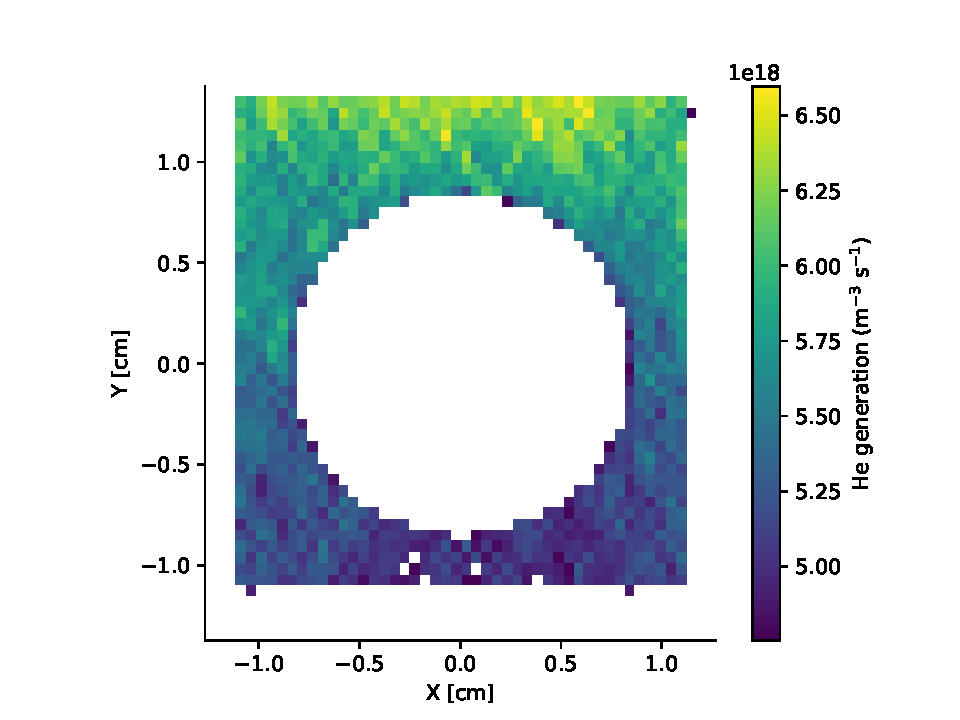
\includegraphics[width=\linewidth]{Figures/Chapter5/helium_transmutation_in_monoblock.pdf}
        \caption{2D distribution.}
    \end{subfigure}%
    \begin{subfigure}{0.5\linewidth}
        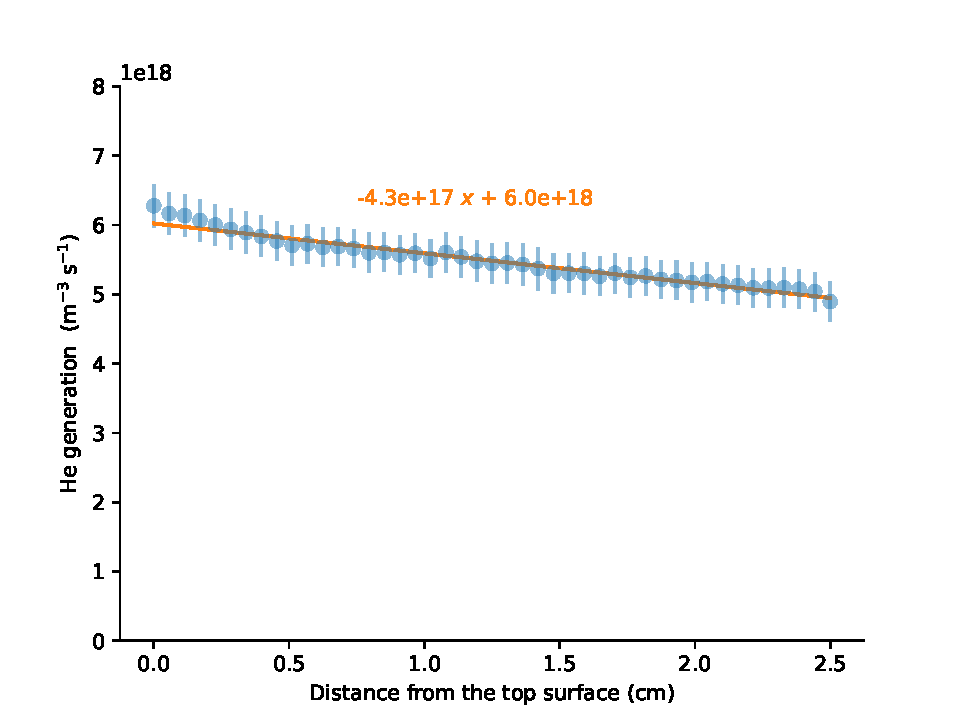
\includegraphics[width=\linewidth]{Figures/Chapter5/he_generation_distribution.pdf}
        \caption{Distribution from the top surface. Errors bars correspond to the 95 \% confidence interval.}
        \labfig{helium generation distribution}
    \end{subfigure}
    \caption{Helium generation via transmutation in a \gls{monoblock} (only tungsten is shown).}
    \labfig{transmutation helium in monoblock}
\end{figure*}

Note that this is a conservative case as the \gls{monoblock} simulated is right below the neutron source.
Other \glspl{monoblock} of the \gls{divertor} will be tilted and shadowed by others and therefore will interact less with the neutrons.


\subsection{Tritium decay}

The generation of helium via tritium decay was computed from \gls{festim} simulations of hydrogen transport in \glspl{monoblock}.
For this case, a volumetric source was added to take the radioactive decay into account.
\refeq{mobile} and \refeq{trapped} can be written as:

\begin{equation}
    \frac{\partial c_\mathrm{m}}{\partial t}=\nabla \cdot (D \nabla c_\mathrm{m} ) -\sum \frac{\partial c_{\mathrm{t}, i}}{\partial t} - \lambda_\mathrm{decay} c_\mathrm{m}
\end{equation}

\begin{equation}
    \frac{\partial c_{\mathrm{t}, i}}{\partial t}=k_i \cdot c_\mathrm{m} \cdot\left(n_{i}-c_{\mathrm{t}, i}\right)-p_i \cdot c_{\mathrm{t}, i} - \lambda_\mathrm{decay} c_{\mathrm{t}, i}
\end{equation}
where $\lambda_\mathrm{decay}$ is the decay constant in \si{s^{-1}}.
The decay constant is expressed from the tritium radioactive half-life $\tau_{1/2}$:
\begin{equation}
    \lambda_\mathrm{decay} = \frac{\ln 2}{\tau_{1/2}} \approx \SI{1.77e-9}{s^{-1}}
\end{equation}

The generation rate of helium from tritium decay is directly proportional to the hydrogen (tritium) retention can therefore be expressed as $\lambda_\mathrm{decay} (c_\mathrm{m} + \sum c_{\mathrm{t}, i})$.
In order to remain conservative, it was computed at steady state.

The maximum generation rate of helium in the \gls{monoblock} was found to be \SI{6.5e12}{m^{-3}.s^{-1}} (see \reffig{he generation from t decay}).
This value assumes all the implanted hydrogen is tritium and should be halved to consider a 50\%-50\% DT mixture.
This is order of magnitudes below the generation from direct implantation.

\begin{figure}
    \centering
    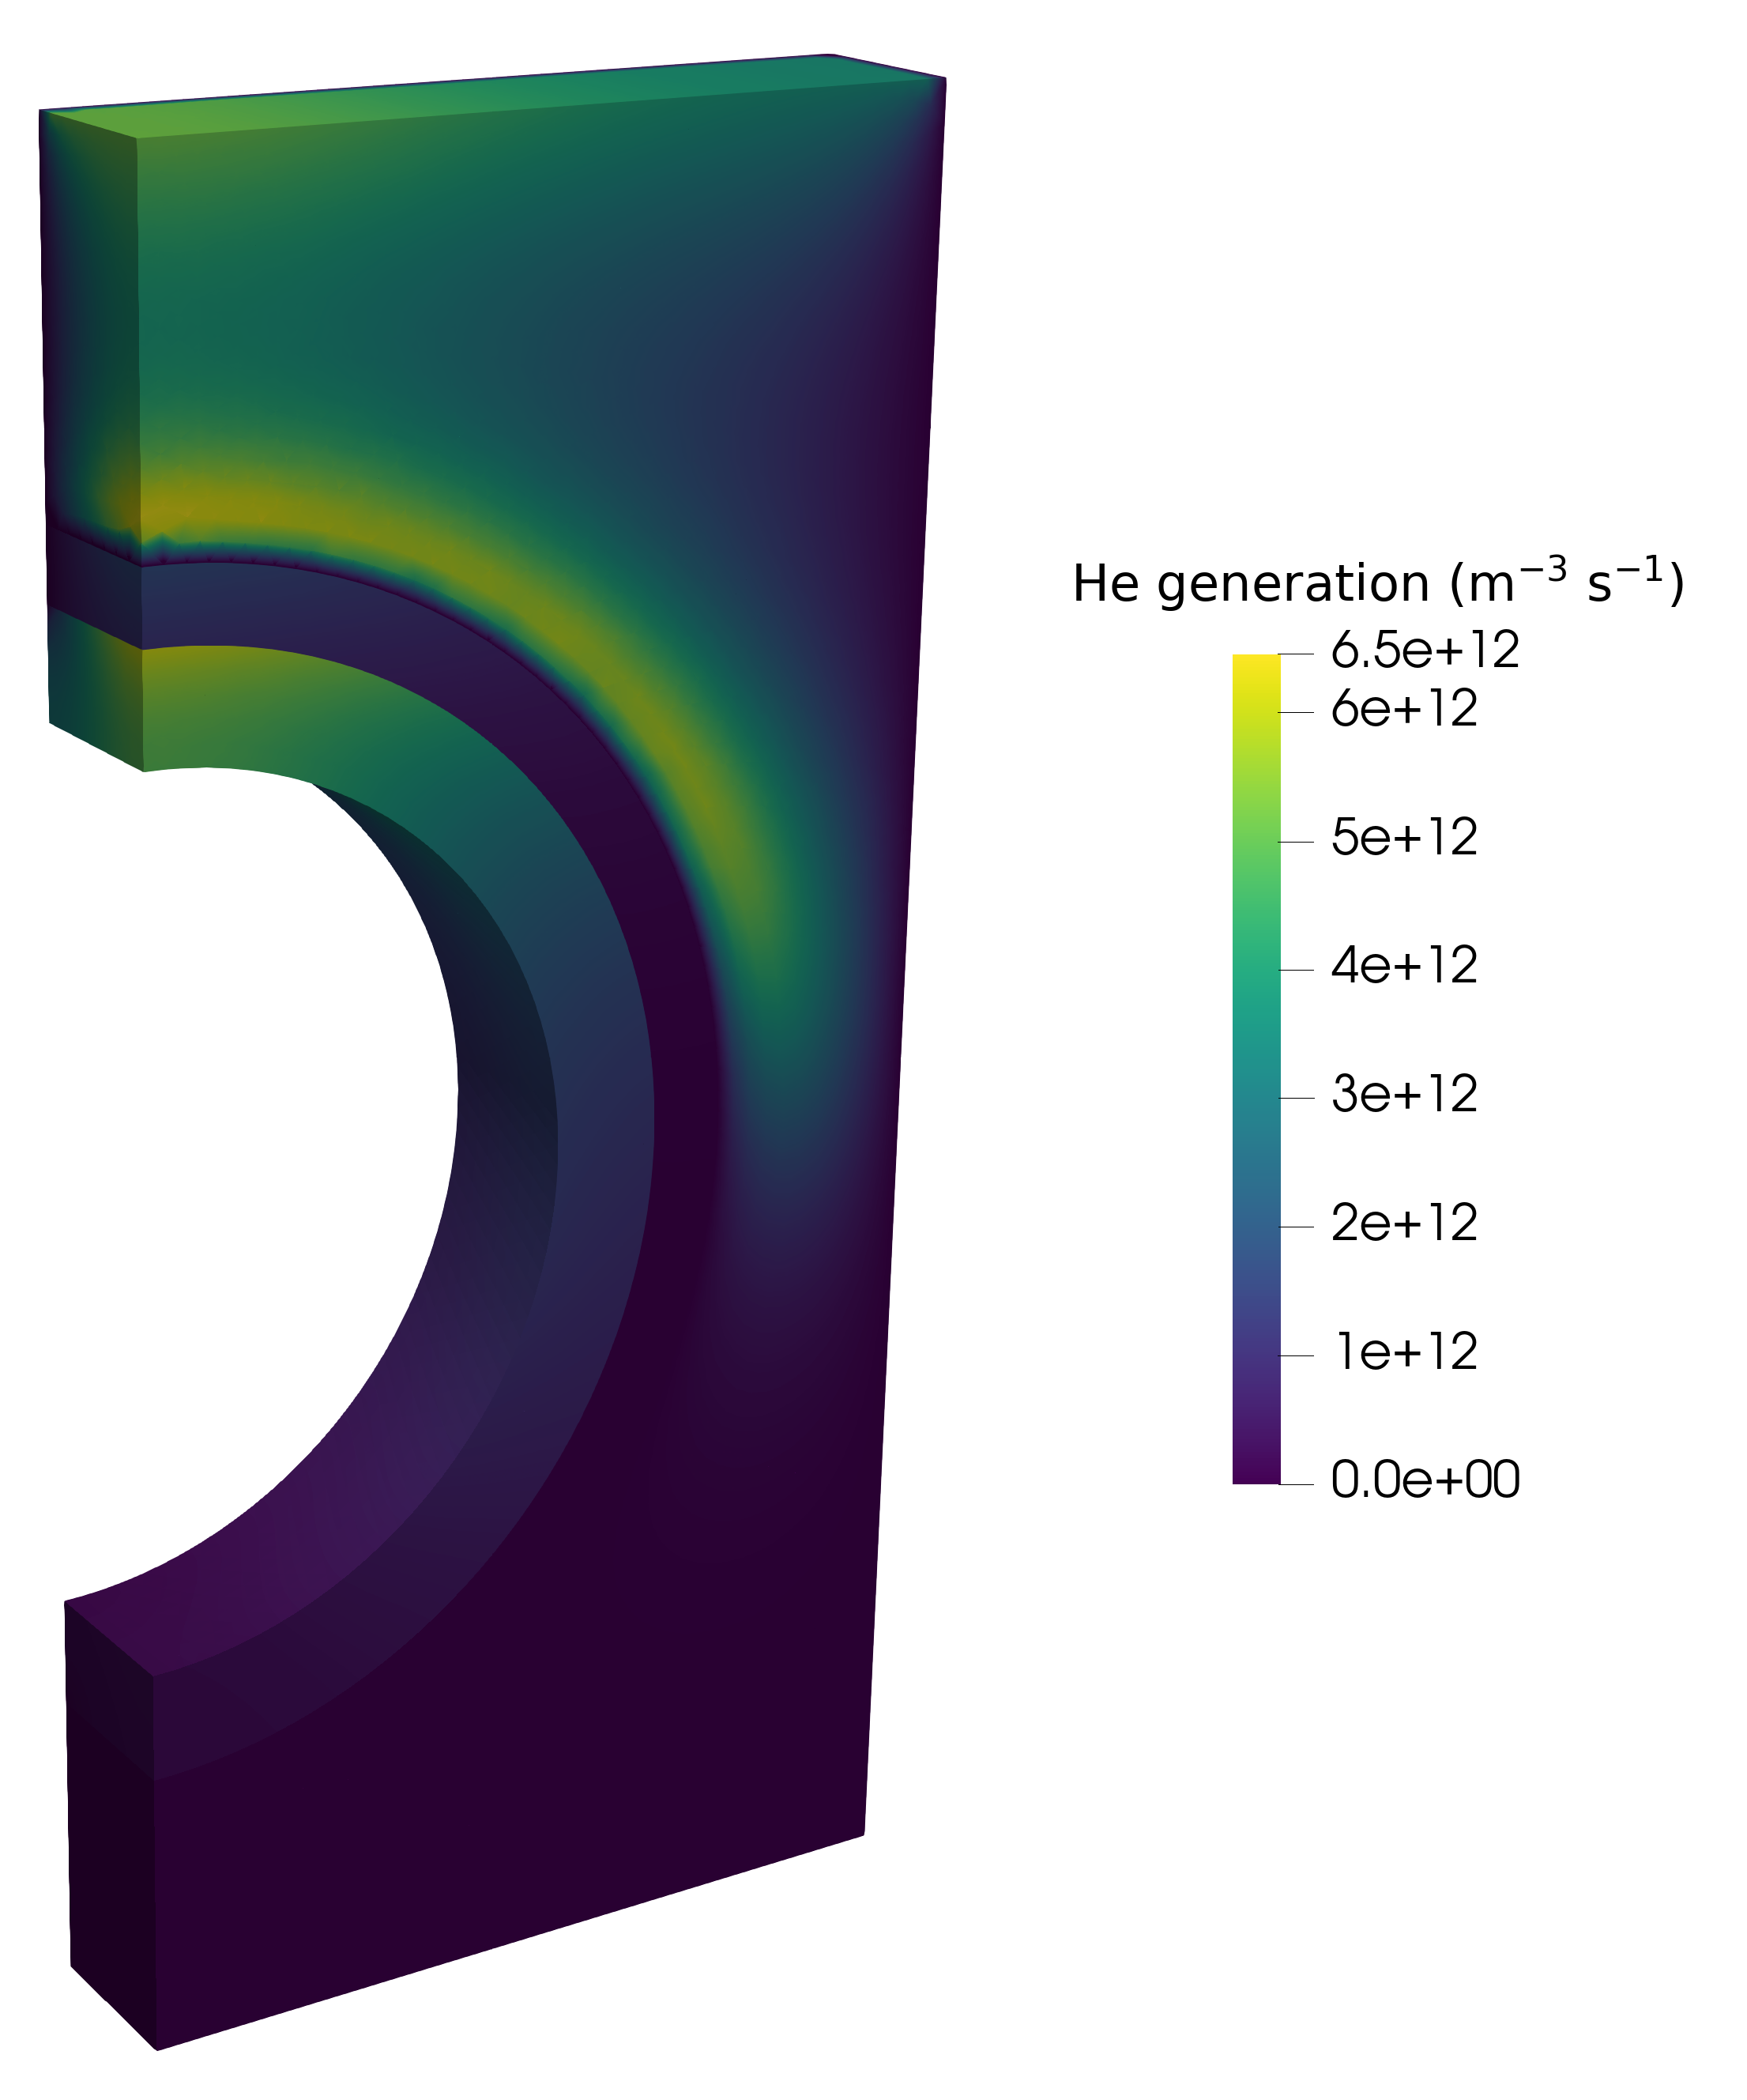
\includegraphics[width=0.5\linewidth]{Figures/Chapter5/he_generation_decay.png}
    \caption{Steady state helium generation from tritium decay in a monoblock.}
    \labfig{he generation from t decay}
\end{figure}


When comparing the production of helium from indirect sources with the quantity helium implanted from the plasma, it appears that the indirect sources are negligible (see \reffig{comparison helium generation}).

\begin{figure}
    \centering
    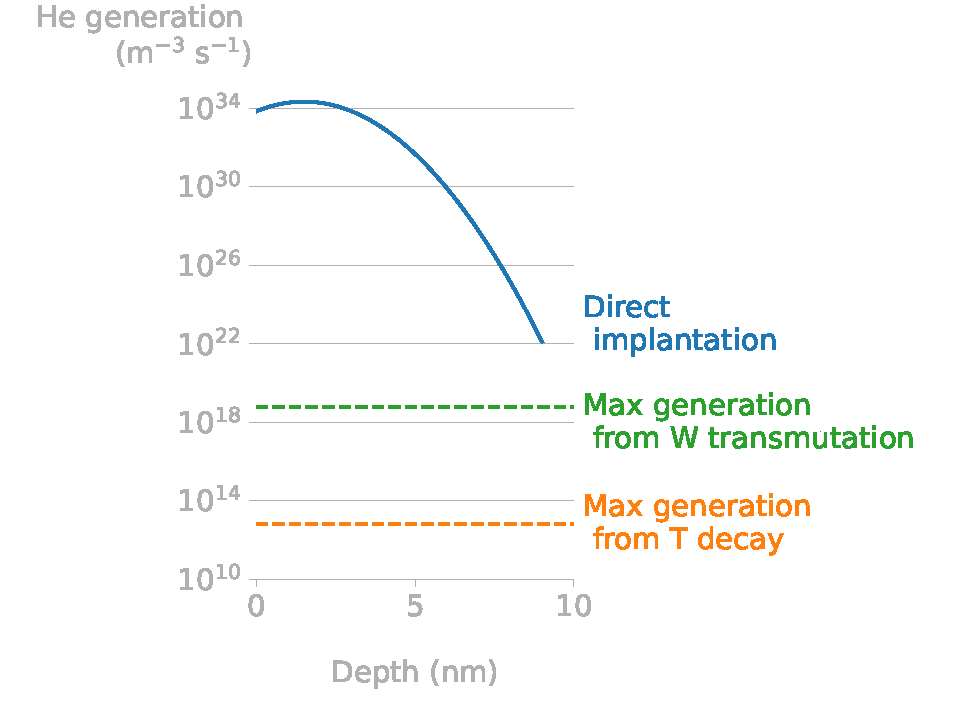
\includegraphics[width=\linewidth]{Figures/Chapter5/helium_generation.pdf}
    \caption{Comparison of the three sources of helium in a \gls{monoblock}. The source from direct implantation was computed for an incident flux of \SI{5e25}{m^{-2}.s^{-1}} with a gaussian distribution (mean of \SI{1}{nm} and standard deviation of \SI{1.5}{nm}).}
    \labfig{comparison helium generation}
\end{figure}

\section{Model description}\labsec{helium model description}
This Section describes the \gls{He} transport model and the grouped approach employed to simplify it.

\subsection{Helium clustering model}

This model describes the evolution of the concentrations of pure interstitial \gls{He} clusters (He$_x$) and mixed \gls{He}-vacancies clusters (He$_x$V$_y$) that are formed by \gls{trap mutation} events.
\begin{figure*}
    \centering
    \begin{overpic}[width=0.7\linewidth]{Figures/Chapter2/He clustering.pdf}
        \put(10, 60){He$_1$}
        \put(25, 60){He$_2$}
        \put(45, 60){He$_3$}
        \put(60, 60){He$_4$}
        \put(85, 60){V$_1$He$_7$}
        \put(78, 15){V$_1$He$_8$}
        \put(50, 15){V$_1$He$_9$}
        \put(22, 15){V$_2$He$_{10}$}
        
    \end{overpic}
    \caption{Representation of \gls{He} clustering in solids. Dissociation is omitted for simplification purposes. The thickness of the grey arrows represents the magnitude of the reaction rate between mobile He$_1$ and other clusters at the same distance.}
    \labfig{clustering sketch}
\end{figure*}


The spatio-temporal evolution of each species of size $i$ is defined by:
\begin{equation}
    \frac{\partial c_i}{\partial t} =  \nabla \cdot (D_i\nabla c_i) + \Gamma_i + R_i
    \labeq{model}
\end{equation}
In Equation \refeq{model}, the first term of the right hand-side is the diffusion term where ${D=D_0 \cdot \exp\big(-E_\mathrm{diff}/ (k_B \cdot T )\big)}$ is the thermally activated diffusion coefficient expressed in \si{m^2.s^{-1}} with $E_\mathrm{diff}$ the diffusion activation energy in \si{eV}, $k_B$ the Boltzmann constant in \si{eV.K^{-1}} and $T$ the temperature in \si{K}.
If a species $i$ is assumed to be immobile, its diffusion coefficient $D_i$ is zero.
$\Gamma_i$ is the external production rate of species $i$.

The term $R_i$ is the coupling term due to reactions between species.
A simple reaction between two species can be described as:
\begin{equation}
    \ce{A + B <=>[k^+_\mathrm{A,B}][k^-_\mathrm{A,B}] AB}
\end{equation}

The forward rate constant $k^+_{A,B}$ is the clustering rate and is calculated using the theory of diffusion-limited reactions \sidecite{goldstein_diffusion_2007}:
\begin{equation}
    k^+_\mathrm{A,B} = 4 \pi (r_\mathrm{A} + r_\mathrm{B}) (D_\mathrm{A} + D_\mathrm{B})
\end{equation}
where $r_\mathrm{A}$ and $r_\mathrm{B}$ are the capture radii and $D_\mathrm{A}$ and $D_\mathrm{B}$ are the diffusion coefficients of species A and B respectively.
The backward rate constant $k^-_\mathrm{A,B}$ is the dissociation rate and is obtained using chemical equilibrium principles \cite{goldstein_diffusion_2007}:
\begin{equation}
    k^-_\mathrm{A,B} =\rho k^+_\mathrm{A,B}e^{\frac{-E_b}{k_B T}}
\end{equation}
where $\rho$ is the atomic density in $\si{m^{-3}}$ ($\rho = \SI{6.3e28}{m^{-3}}$ for W), $k_B$ is the Boltzmann constant in \si{eV.K^{-1}}, $T$ is the temperature in \si{K} and $E_b$ is the binding energy for the reaction \ce{AB -> A + B} in \si{eV}.

The reaction term $R_i$ is the coupling term between concentrations and is expressed as:

\begin{equation}
    R_i=  \sum_{m} k^+_{m,i-m} c_m c_{i-m}  - c_i \sum_m \left( k_{i, m}^+ c_{m} + k_{i+1}^- c_{i+1} -  k_i^- c_i \right)
    \labeq{reaction term}
\end{equation}


In Equation \refeq{reaction term}, $c_i$ is the concentration of clusters of size $i$ in \si{m^{-3}}.
The first term corresponds to the reactions producing clusters of size $i$.
The second one corresponds to the ones reacting with clusters of size $i$.
The third term accounts for bigger clusters dissociating.
Finally, the last term corresponds to clusters of size $i$ dissociating.

\subsection{Grouped approach}
Extending this clustering model to clusters containing millions of helium extremely increases the computational cost.
A grouped approach proposed by Faney et al.\ \sidecite{faney_spatially_2014} for reducing the number of equations will therefore be employed.
This technique consists in grouping the big clusters that have a similar behaviour in a single equation while explicitly accounting for smaller clusters.

The clustering equations can be written as follows:

\begin{subequations}
    \begin{align}
        \frac{\partial c_1}{\partial t} &= \nabla \cdot (D_1 \nabla c_1) + \Gamma + \sum\limits_{i=2}^N k_{i}^- c_i - 2k_{1, 1}^+ c_1^2 - \sum\limits_{i=2}^N k_{1,i}^+ c_1 c_i - \sum\limits_{i=N+1}^\infty k_{1,i}^+ c_1 c_i \\
        \frac{\partial c_2}{\partial t} &= \nabla \cdot (D_2 \nabla c_2) - k_{1, 2}^+ c_1 c_2 + k_{1, 1}^+ c_1^2 - k_{2}^- c_2 + k_{3}^- c_3\\
        \vdots \nonumber\\
        \frac{\partial c_i}{\partial t} &= - k_{1, i}^+ c_1 c_i + k_{1, i-1}^+ c_1 c_{i-1} - k_{i}^- c_i\\
        \frac{\partial c_{i+1}}{\partial t} &= - k_{1, i+1}^+ c_1 c_{i+1} + k_{1, i}^+ c_1 c_i\\
        \vdots \nonumber
    \end{align}
    \labeq{temporal evolution no grouping}
\end{subequations}
where $N$ is some threshold required for the grouping technique.

In order to simplify this model, the following quantities are defined:

\begin{align}
    c_b &= \sum\limits_{i=N+1}^\infty c_i \quad \text{ : total concentration of clusters containing more than $N$ He} \\
    \langle i_b \rangle &= \frac{1}{c_b} \sum\limits_{i=N+1}^\infty i c_i \quad \text{ : average He content in $c_b$} \\
    \langle r_b \rangle &=  \frac{1}{c_b}\sum\limits_{i=N+1}^\infty r_i c_i \quad \text{ : average radius in $c_b$}\\
    \langle k_b^+ \rangle &=  \frac{1}{c_b}\sum\limits_{i=N+1}^\infty k_{1,i}^+ c_i = 4 \pi D_1 (r_1 + \langle r_b \rangle) \quad \text{ : average clustering rate in $c_b$}
\end{align}

Clusters with more than $N$ \gls{He} ($c_b$) will be referred as ``bubbles'' in the following.

Equation \refeq{temporal evolution no grouping} therefore reads:

\begin{subequations}
    \begin{align}
        \frac{\partial c_1}{\partial t} &= \nabla \cdot (D_1 \nabla c_1) + \Gamma + \sum\limits_{i=2}^N k_{i}^- c_i- 2k_{1, 1}^+ c_1^2 - \sum\limits_{i=2}^N k_{1,i}^+ c_1 c_i - \langle k_b^+ \rangle c_1 c_b \\
        \frac{\partial c_2}{\partial t} &= \nabla \cdot (D_2 \nabla c_2) - k_{1, 2}^+ c_1 c_2 + k_{1, 1}^+ c_1^2 - k_{2}^- c_2 + k_{3}^- c_3\\
        \vdots \nonumber\\
        \frac{\partial c_N}{\partial t} &= - k_{1, N}^+ c_1 c_N + k_{1, N-1}^+ c_1 c_{N-1} - k_{N}^- c_N\\
        \frac{\partial c_b}{\partial t} &= k_ {1,N}^+ c_1 c_N \\
        \frac{\partial (\langle i_b \rangle c_b)}{\partial t} &= (N+1)k_ {1,N}^+ c_1 c_N  + \langle k_b^+ \rangle c_1 c_b
    \end{align}
    \labeq{temporal evolution grouping}
\end{subequations}

The mean radius of pure \gls{He} clusters \sidecite{faney_spatially_2015} is given by:
\begin{equation}
    r_{\mathrm{He}_x} = r_{\mathrm{He}_1} + \left(\frac{3}{4\pi} \frac{a_0^3}{10} x \right)^{1/3} - \left( \frac{3}{4\pi} \frac{a_0^3}{10} \right)^{1/3}
    \labeq{radius pure He}
\end{equation}
with $r_{\mathrm{He}_1} = \SI{0.3}{nm}$.

Several assumptions are made:
\begin{itemize}
    \item The average radius is assumed to be a function of $\langle i_b \rangle$:
    \begin{equation}
        \begin{split}
            \langle r_b \rangle &= r(\mathrm{He}_{\langle i_b \rangle}\mathrm{V}_{\langle i_b \rangle/4}) \\
            &= r_{\mathrm{He}_0 \mathrm{V}_1} + \left(\frac{3}{4 \pi} \frac{a_0^3}{2} \frac{\langle i_b \rangle}{4} \right)^{1/3} - \left(\frac{3}{4 \pi} \frac{a_0^3}{2} \right)^{1/3}
        \end{split}
        \labeq{radius average}
    \end{equation}
    with $a_0 = \SI{0.318}{nm}$ the lattice parameter and $r_{\mathrm{He}_0 \mathrm{V}_1} =  a_0 \sqrt{3}/4$.
    The average radius $\langle r_b \rangle$ is assumed to be only dependent on $\langle i_b \rangle$.
    The number of vacancies in bubbles is assumed to be $\langle i_b \rangle/4$.
    This assumption is motivated by \gls{md} computations showing that \gls{trap mutation} events occur for every four additional helium in large \gls{vacancy}-helium clusters.
    Moreover, theoretical models for He bubbles growth in metal suggest a similar trend \sidecite{hammond_theoretical_2020}.
    \item Dissociation of large clusters is neglected (i.e.\ $k_i^- = 0$ for $i>N$).
    Indeed, the activation energy for \gls{trap mutation} events is lower than that of He or \gls{vacancy} emission\sidecite{boisse_modeling_2014}. Dissociation of large clusters by \gls{vacancy} or He emission is therefore negligible.
\end{itemize}

The current implementation further simplifies Faney's model \sidecite{faney_spatially_2014}:
\begin{itemize}
    \item Interactions with \gls{self-interstitial} atoms or pre-existing vacancies are not taken into account.
    In this work, the only dissociations are He emissions from small mobile clusters and \gls{trap mutation} for large clusters.
    It was showed that this assumption did not have an impact on the results (see \reffig{tendril profiles}).
    \item The only clusters explicitly computed are $\mathrm{He}_{x \leq 6}$ (i.e.\ $N=6$) whereas Faney's work explicitly accounted for clusters up to $\mathrm{V}_{50}\mathrm{He}_{250}$ and solved a bigger system of equations.
    The influence of this threshold $N$ above which clusters are integrated in the quantity $c_b$ is discussed in \refsec{impact of N}.
    \item Clusters containing more than six \gls{He} atoms are assumed to be immobile (i.e.\ $D_i = 0$ for $i>6$) due to \gls{trap mutation} events.
    This assumption is motivated by \gls{dft} and \gls{md} results suggesting that the \gls{self-trapping} energy is below the binding energy of one He atom in a pure He cluster for clusters containing more than five He atoms \sidecite{boisse_modeling_2014}.

    For smaller clusters ($\mathrm{He}_1$, $\mathrm{He}_2$,$\ldots$, $\mathrm{He}_6$) the diffusion coefficient and the dissociation by He emission energy vary with the number of \gls{He} atoms in the cluster (see \reftab{clusters properties}).
\end{itemize}

\begin{table}
    \centering
    \begin{tabular}{L{1cm} R{2cm} R{1.6cm} R{1.1cm} R{1.6cm} R{1.1cm} R{2cm}}
        Cluster & $D_0 (\si{m^2 s^{-1}})$  & $E_\mathrm{diff} (\si{eV})$ &  $E_b (\si{eV})$   \\
        \hline
        \\
        He$_1$ & $2.95\times 10^{-8}$ & $0.13$ & - \\
        He$_2$ & $3.24\times 10^{-8}$ & $0.20$ & 1.0\\
        He$_3$ & $2.26\times 10^{-8}$ & $0.25$ & 1.5\\
        He$_4$ & $1.68\times 10^{-8}$ & $0.20$ & 1.5\\
        He$_5$ & $5.20\times 10^{-9}$ & $0.12$ & 1.6\\
        He$_6$ & $1.20\times 10^{-9}$ & $0.30$ & 2.0\\
    \end{tabular}
    \caption{Pure \gls{He} clusters properties in \gls{W}. Diffusion properties are taken from Faney et al.\ \cite{faney_spatially_2015} and binding energies are taken from Becquart et al.\ \cite{becquart_microstructural_2010}.}
    \labtab{clusters properties}
\end{table}

% for some reason, uncommenting this activates the top table
% \begin{table}
%  \begin{tabular}{ c c c c }
%  \toprule
%  col1 & col2 & col3 & col 4 \\
%  \midrule
%  \multirow{3}{4em}{Multiple row} & cell2 & cell3 & cell4\\ &
%  cell5 & cell6 & cell7 \\ &
%  cell8 & cell9 & cell10 \\
%  \multirow{3}{4em}{Multiple row} & cell2 & cell3 & cell4 \\ &
%  cell5 & cell6 & cell7 \\ &
% cell8 & cell9 & cell10 \\
%  \bottomrule
%  \end{tabular}
% \end{table}


This \gls{He} transport model was implemented in Python and solved using the finite element solving platform \gls{fenics} \sidecite{alnaes_fenics_2015}.


\section{Verification \& Validation}
\subsection{Code comparison: Tendril case} \labsec{tendril case}

\begin{figure*}
    \centering
    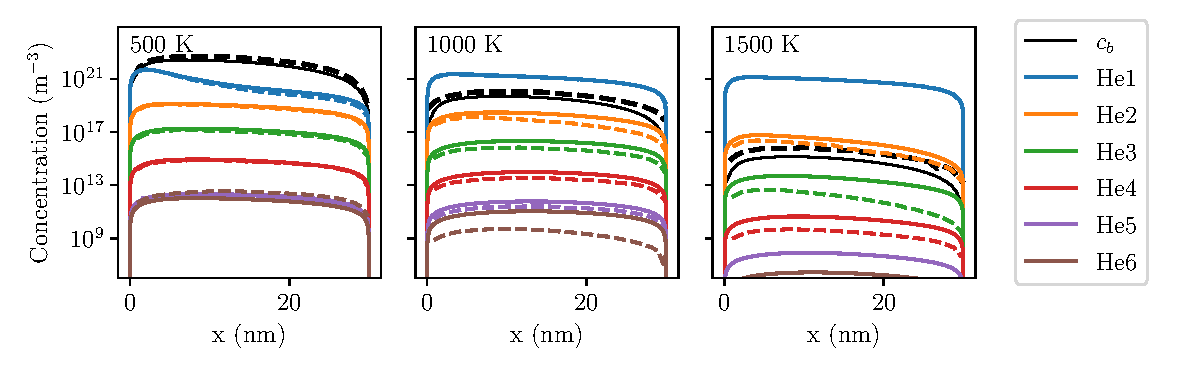
\includegraphics[width=\linewidth]{Figures/Chapter4/profiles_tendrils.pdf}
    \caption{He clusters concentration profiles in the \gls{tendril} at \SI{500}{K}, \SI{1000}{K} and \SI{1500}{K} under \SI{100}{eV} He exposure at \SI{1e22}{m^{-2}.s^{-1}} at a fluence of \SI{5e25}{m^{-2}}. Comparison between the current implementation (solid) and Faney's results \cite{faney_spatially_2015} (dashed).}
    \labfig{tendril profiles}
\end{figure*}

The current implementation was compared to literature results\cite{faney_spatially_2015}.
Helium exposure in a \gls{tendril} was simulated in 1D.
The helium flux is \SI{1e22}{m^{-2}.s^{-1}} and the fluence was \SI{5e25}{m^{-2}}.

The domain size is \SI{30}{nm} and the volumetric source term is described as follows:
\begin{equation}
    \Gamma(x) = \varphi_\mathrm{imp} \; f(x) 
\end{equation}
where $\varphi_\mathrm{imp} = \SI{1e22}{m^{-2} s^{-1}}$ is the implanted He flux and $f(x)$ is a Gaussian distribution with a mean value $\mu = R_p = \SI{1.5}{nm}$ and a standard deviation $\sigma = \SI{1}{nm}$ which corresponds to a \SI{100}{eV} He implantation based on \gls{srim} computations \sidecite{ziegler_srim_2010}.

Mobile He clusters concentrations were set to zero at the \gls{tendril}'s surfaces ($x=\SI{0}{nm}$ and $x=\SI{30}{nm}$).

Concentration profiles computed by the current implementation showed good agreement with the ones obtained by Faney et al.\ \cite{faney_spatially_2015} (see \reffig{tendril profiles}).
The discrepancies are likely due to a difference in the set of dissociation energies that have been used as these energies have an impact on the concentration profiles (see \reffig{parametric study dissociation energies}).
Indeed, at low temperature, where dissociation is not activated, the discrepancies were rather small whereas at high temperature, differences increased because dissociation became more dominant.

\begin{figure*}
    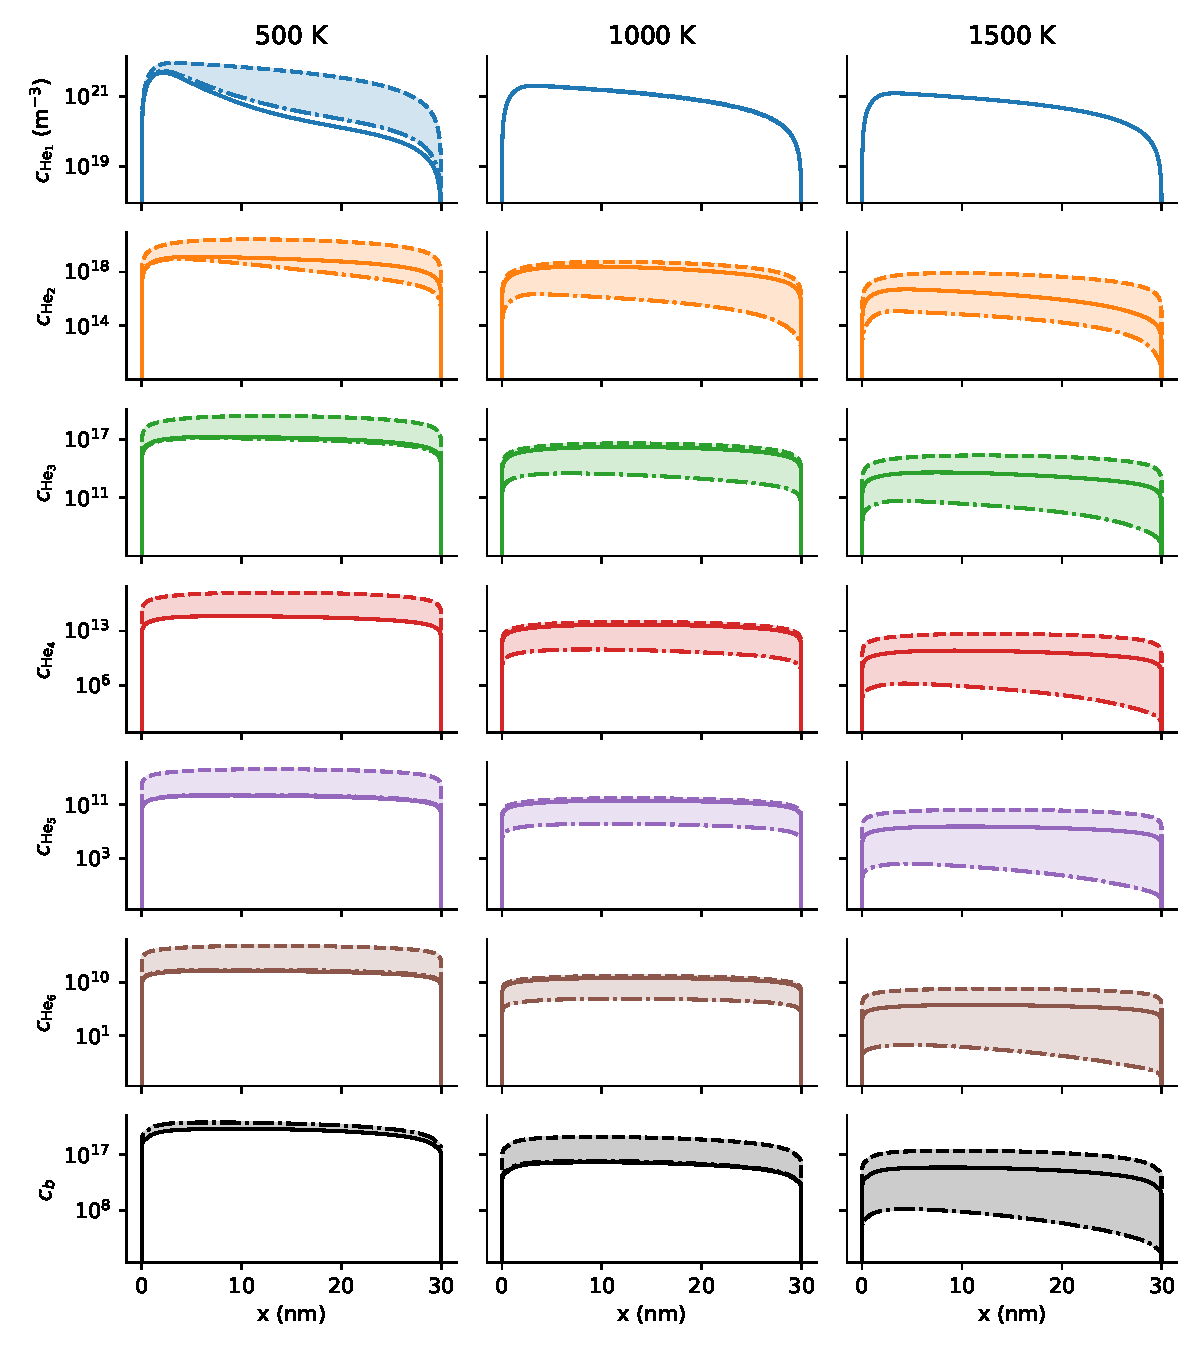
\includegraphics[width=\linewidth]{Figures/Chapter5/parametric_study_dissociation_energies.pdf}
    \caption{Helium clusters concentration profiles on the tendril case with dissociation energies varying from -\SI{0.5}{eV} (dash-point) to +\SI{0.5}{eV} (dash).}
    \labfig{parametric study dissociation energies}
\end{figure*}

% When $c_b$ is small compared to $c_{\mathrm{He}_1}$, the equilibrium of $\mathrm{He}_1$ is independent of these dissociation energies and the profiles for $\mathrm{He}_1$ are identical.

Moreover, increasing the temperature tended to inhibit bubble formation in the \gls{tendril}.
This was explained by a greater increase in the dissociation rate and in losses at surfaces than the increase in the clustering rate.
This observation is in agreement with \gls{md} results simulating He implantation in \glspl{tendril} \sidecite{wei_better_2020, wei_understanding_2019}.
The current implementation and the additional assumptions that were made are therefore valid.

\subsection{Comparison with experiments}

\begin{figure} [h]
    \centering
    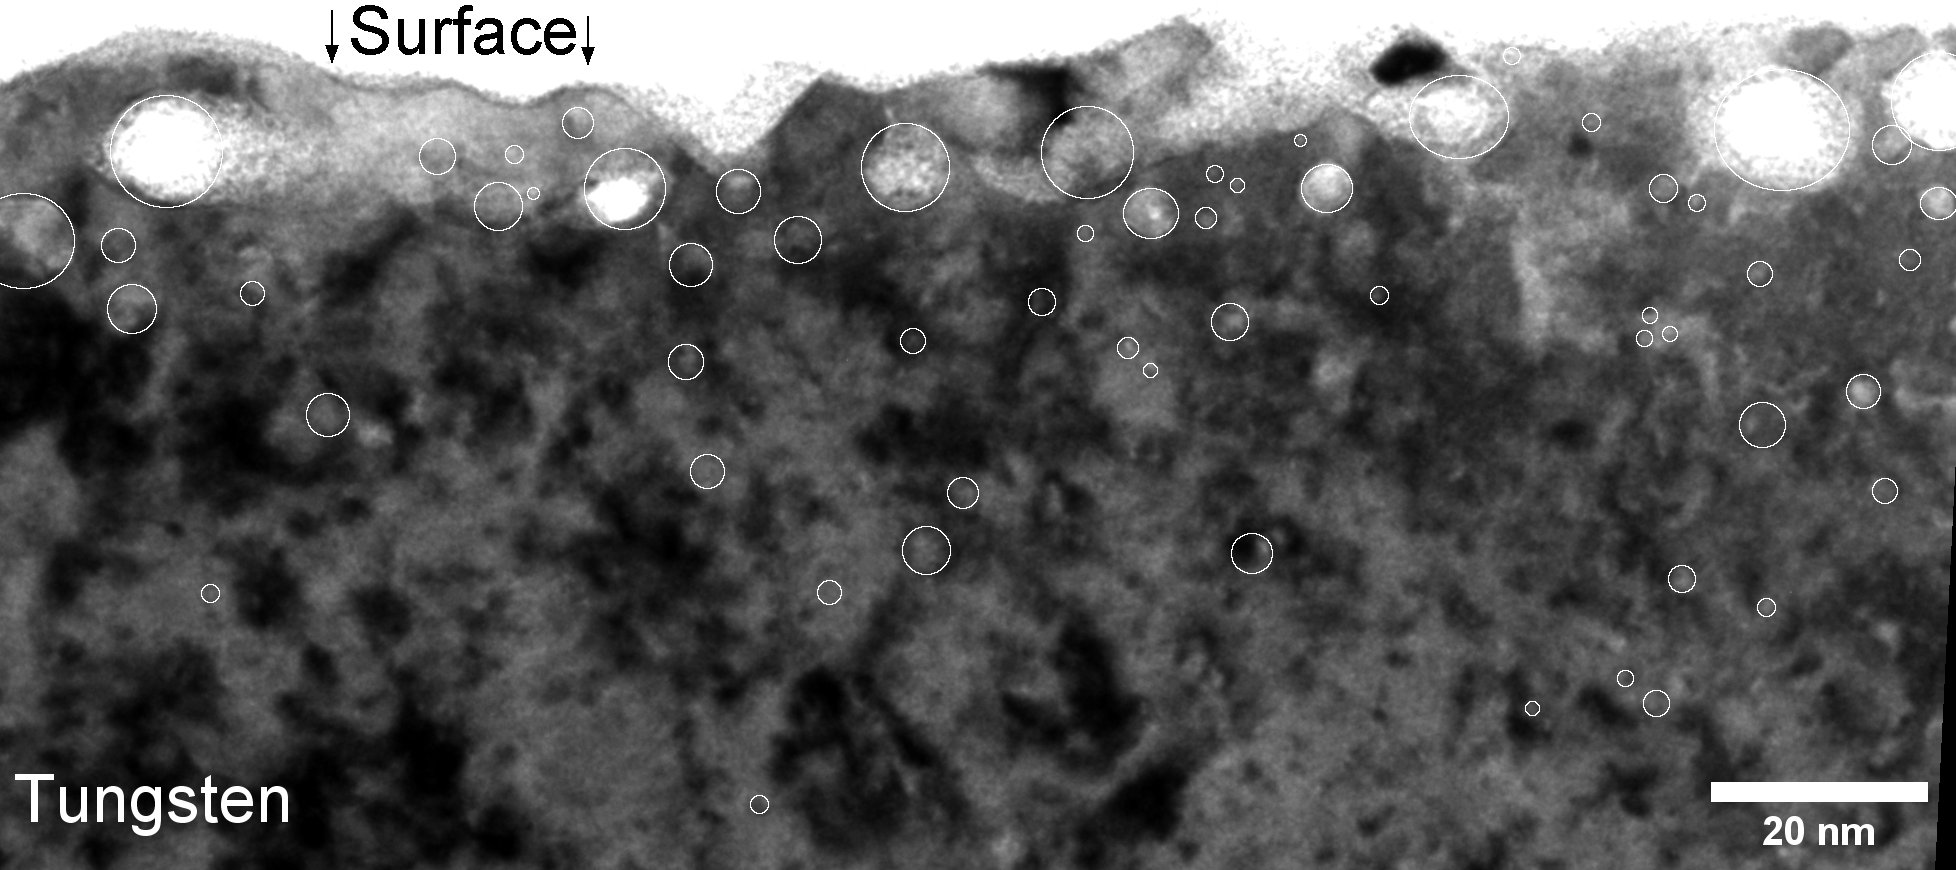
\includegraphics[width=\linewidth]{Figures/Chapter4/bubbles_tem.jpg}
    \caption{\gls{tem} images of W after exposure to \SI{75}{eV} He at \SI{2.3e22}{m^{-2}.s^{-1}} and \SI{1053}{K} for \SI{13}{s} showing bubbles that have burst, large size bubbles at the near surface and small size bubbles in the bulk.}
    \labfig{tem images}
\end{figure}

\begin{figure} [h!]
    \centering
    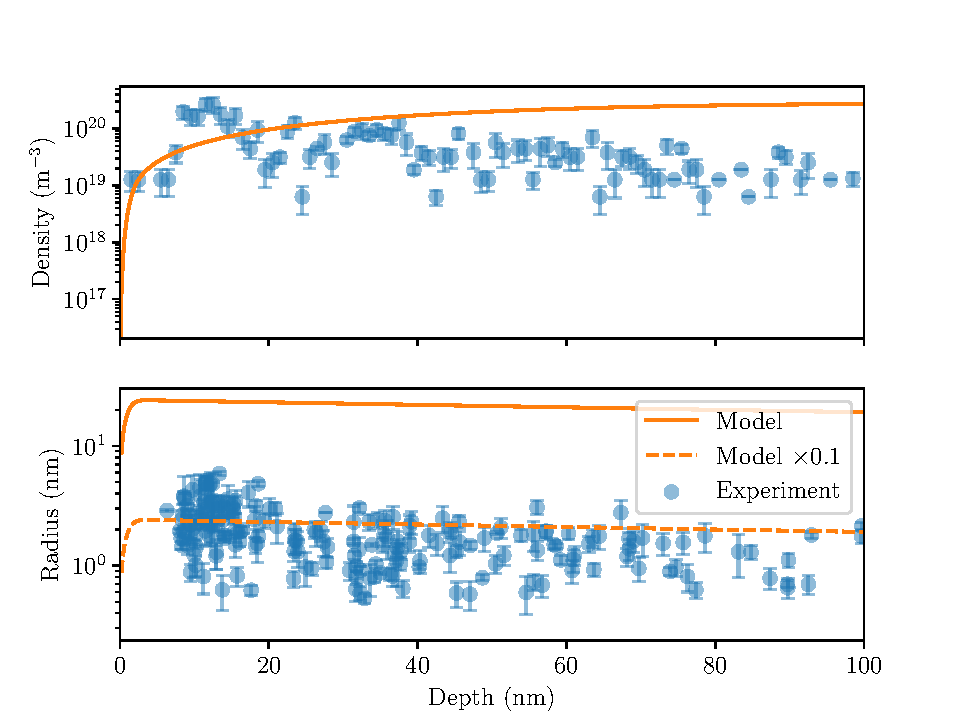
\includegraphics[width=\linewidth]{Figures/Chapter4/comparison_model_exp.pdf}
    \caption{Comparison of experimental results with simulations for W implanted with \SI{75}{eV} He at \SI{2.3e22}{m^{-2}.s^{-1}} and \SI{1053}{K} for \SI{13}{s}. Error bars correspond to the lowest and highest radius in the \gls{tem} image.}
    \labfig{exp model comparison}
\end{figure}

% He implantation experiments were performed on W and TEM (Transmission Electron Microscopy) images were produced (see \reffig{tem images}).
% W was irradiated with \SI{75}{eV} He at \SI{2.3e22}{m^{-2}.s^{-1}} and \SI{1053}{K} for \SI{13}{s}.
% Comparison of under- and over-focused TEM images allowed identification of the bubbles.
% say something about the imaging technique or the lamella...

He implantation experiments were performed on W in the linear plasma device PSI--2 \sidecite{kreter_linear_2015}.
W was irradiated with \SI{75}{eV} He at \SI{2.3e22}{m^{-2}.s^{-1}} and \SI{1053}{K} for \SI{13}{s}.
A thin lamella for cross-sectional observations was prepared using the \gls{fib} technique with a Dual Beam FIB (FEI Helios 600 NanoLab).
Prior to \gls{fib} cutting, the surface of the sample was coated with a SiO layer for better contrast and then with a protective platinum layer to avoid damaging the surface during the lamella preparation.
Cross-sectional observations of the He-implanted W were performed using \gls{tem} in a TEM FEI Titan 80-300 apparatus.

A typical \gls{tem} image of the lamella is presented in \reffig{tem images}.
Comparison of under- and over-focused \gls{tem} images allowed identification of the bubbles.
Bubbles were observed up to \SI{100}{nm} with larger bubbles closer to the surface and smaller bubbles deeper in the bulk.
Open bubbles and holes at the surface were also observed suggesting bursting events occurred.
This is in accordance with what was observed in the simulations (see \reffig{profiles rb half slab}).

A procedure was developed to automate the bubble detection on \gls{tem} images using the ImageJ software \sidecite{schindelin_fiji_2012}.
The area of bubbles were computed as well as their diameter assuming a spherical shape for the bubbles.
Bubble density and size as a function of depth was therefore computed using 12 pairs of under- and over-focused \gls{tem} images.
The bubble density was found to range from \SI{7e19}{m^{-3}} to \SI{2e20}{m^{-3}} and the bubble radius ranged between \SI{1}{nm} and \SI{10}{nm} (see \reffig{exp model comparison}).
Although the resolution of the \gls{tem} is below \SI{1}{nm}, the number of bubbles with radius below \SI{2}{nm} is underestimated due to the limited contrast.

This experiment was simulated using the same exposure conditions.
The simulated bubbles density $c_b$ was found to be in accordance with the one measured experimentally.
Some discrepancies were found at the near surface.

The bubble radius $\langle r_b \rangle$ is however overestimated by an order of magnitude compared to experimental measurements.
This could imply that the current model linking the He content to the bubble radius is overestimated and that a more accurate one is needed.
Bursting in over-pressurised bubbles close to the surface would also reduce the bubble size. 
Finally, it would be worth investigating this further to determine the impact of initial defects.


\section{Bubble growth study}
In this Section, the current implementation is first compared with the one from Faney \sidecite{faney_spatially_2015} to ensure the additional assumptions do not produce different results.
A standard half-slab case is then described and a parametric study is performed by varying the exposure conditions.
Finally, the model is compared against experimental data.

\subsection{Half-slab case} \labsec{half slab}

\begin{figure}
    \centering
    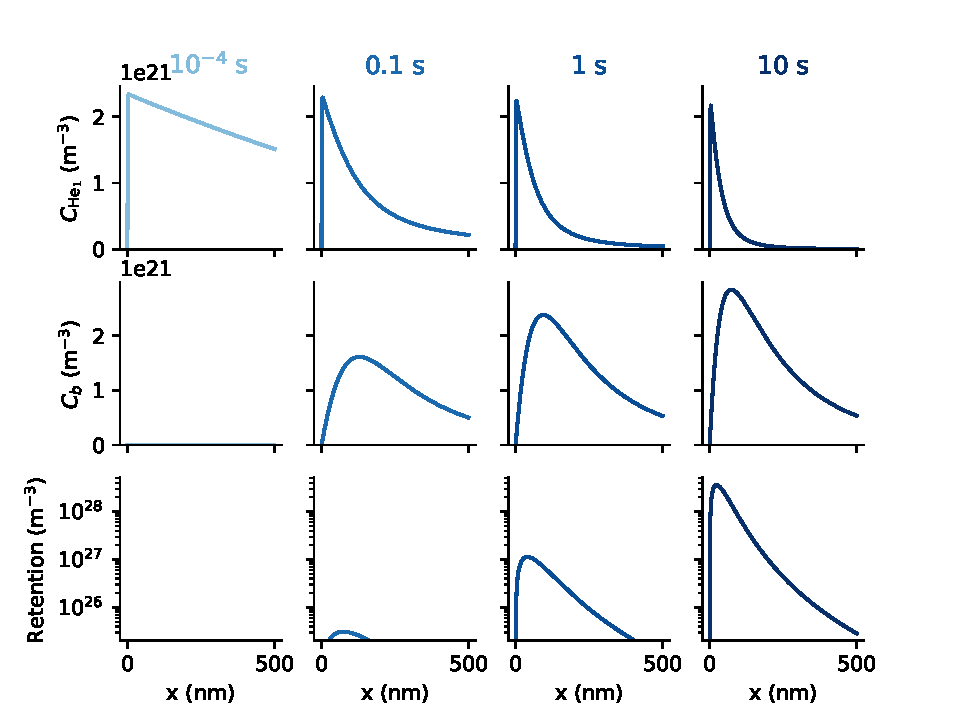
\includegraphics[width=\linewidth]{Figures/Chapter4/half_slab/profiles_half_slab.pdf}
    \caption{Concentration profiles of He$_1$ (left) and bubbles (right) in W exposed to \SI{100}{eV} He at \SI{e22}{m^{-2}.s^{-1}} and \SI{1000}{K}.}
    \labfig{profiles half slab}
\end{figure}

\gls{He} transport was simulated in a 1D semi-infinite \gls{W} slab.
This case is the standard case describing the main quantities of interest of the parametric study performed in \refsec{parametric study}.

The domain size is \SI{0.1}{mm} which is much greater than the penetration depth of \gls{He} in the simulations.
\SI{100}{eV} \gls{He} were implanted in the first \SI{1.5}{nm} as in \refsec{tendril case}.
The implanted flux was \SI{1e22}{m^{-2} s^{-1}} and the temperature was \SI{1000}{K}.

At low \glspl{fluence}, \gls{He} diffused really quickly into the bulk (see \reffig{profiles half slab}) and the bubbles' concentration $c_b$ was found to be zero.
As the \gls{fluence} increased, bubbles started to appear and acted as strong sinks for mobile \gls{He}.
This lead to a great decrease in the mobile He concentration profile.

It is worth noticing the maximum of $c_b$ was not located at the maximum of $c_{\mathrm{He}_1}$ which is the implantation depth $R_p$.
This was explained by the \gls{diffusion} of small mobile clusters as shown by analytical models \sidecite{krasheninnikov_helium_2014}.
As \gls{He} clusters, small mobile clusters diffuse deeper into the bulk until \gls{trap mutation} occurs and bubbles nucleons (clusters with more than 6 \gls{He}) are created.
From that point, bubbles are formed relatively far from the surface.
Because \gls{He} is implanted in the first nanometres, $c_{\mathrm{He}_1}$ is maximum at $R_p = \SI{1.5}{nm}$ and interactions with bubbles are stronger in this region.
This tends to draw the maximum location of $c_b$ towards the surface.

The \gls{He} content in bubbles $\langle i_b \rangle$ and the radius $\langle r_b \rangle$ were computed.
After \SI{10}{s} of implantation, bubbles located in the near surface contained up to \SI{3e7}{He}.
The maximum of $\langle r_b \rangle$ was found to be very close to the surface at approximately \SI{2}{nm} (see \reffig{profiles rb half slab}).
This is explained by the high concentration of mobile \gls{He} in this near surface region.
Moreover, a bursting zone can be defined by the region where $\langle r_b \rangle$ is greater than the depth of the bubble.
In this region, bubble of this size would have likely burst.
% This result was in good agreement with the He bubbles observations performed by Ialovega et al.\ on W \sidecite{ialovega_hydrogen_2020}.

\begin{figure} [h]
    \centering
    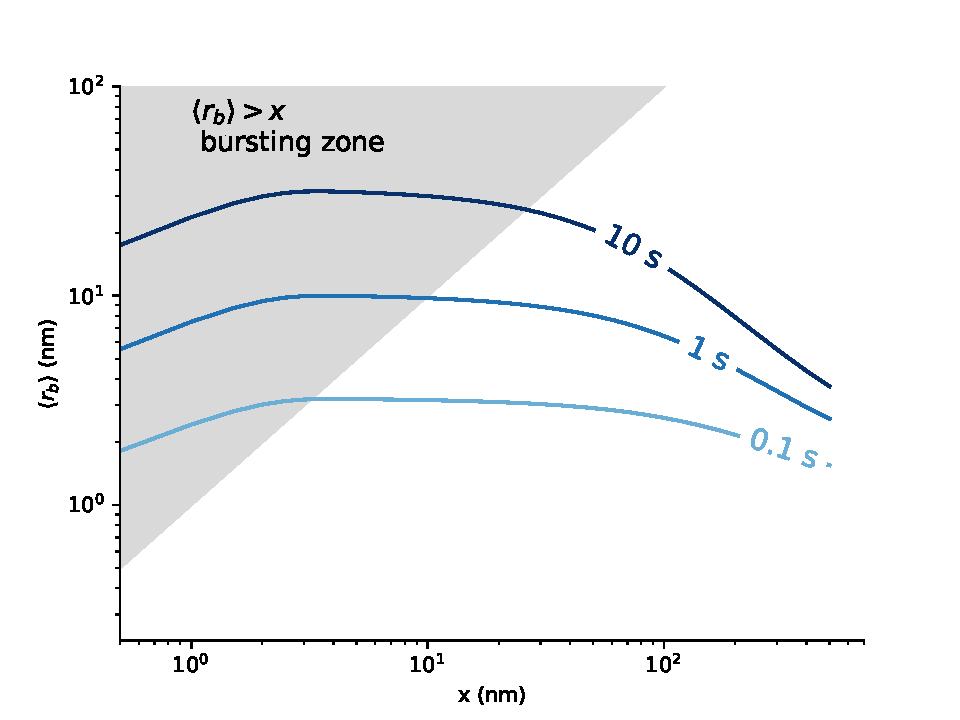
\includegraphics[width=\linewidth]{Figures/Chapter4/half_slab/profile_rb.pdf}
    \caption{Profile of mean bubble radius $\langle r_b \rangle$ as a function of depth $x$ in \gls{W} exposed to \SI{100}{eV} \gls{He} at \SI{e22}{m^{-2}.s^{-1}} and \SI{1000}{K}.}
    \labfig{profiles rb half slab}
\end{figure}

\begin{figure*}
    \centering
    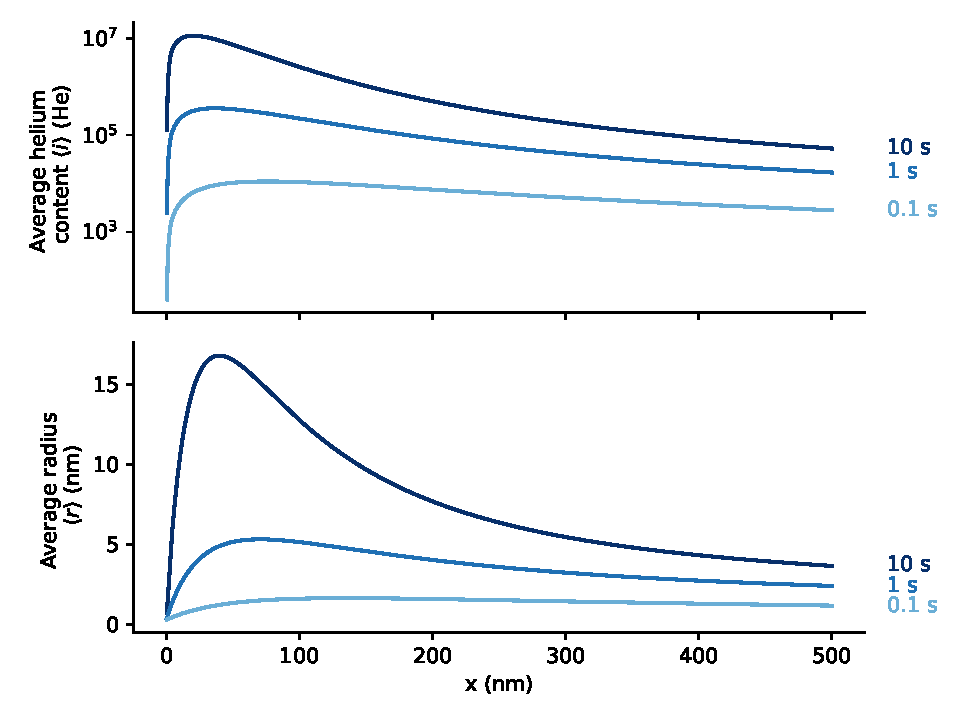
\includegraphics[width=0.75\linewidth]{Figures/Chapter4/half_slab/average_content_radius.pdf}
    \caption{Average helium content $\langle i \rangle$ and average radius $\langle r \rangle$ in all clusters (mobile and bubbles) in \gls{W} exposed to \SI{100}{eV} \gls{He} at \SI{e22}{m^{-2}.s^{-1}} and \SI{1000}{K}.}
    \labfig{content and radius}
\end{figure*}

From this average \gls{He} content in bubbles and from \refeq{radius average} and \refeq{radius pure He} expressing the clusters radii, the average radius $\langle r \rangle$ can be computed as:

\begin{equation}
        \langle r \rangle = \frac{\sum\limits_{i=1}^\infty c_i r_i}{\sum\limits_{i=1}^\infty c_i}
        = \frac{\sum\limits_{i=1}^N c_i r_i + c_b \langle r_b \rangle }{\sum\limits_{i=1}^N c_i + c_b}
\end{equation}

The average content of \gls{He} in all clusters $\langle i \rangle$ is computed similarly:
\begin{equation}
        \langle i \rangle = \frac{\sum\limits_{i=1}^\infty c_i i}{\sum\limits_{i=1}^\infty c_i}
        = \frac{\sum\limits_{i=1}^N c_i i + c_b \langle i_b \rangle }{\sum\limits_{i=1}^N c_i + c_b}
\end{equation}

These two quantities are comparable to the ones obtained by Faney et al.\ \sidecite{faney_spatially_2015}.
After \SI{100}{s} of exposure, the average radius \SI{50}{nm} below the surface was above \SI{10}{nm} (see \reffig{content and radius}).
Moreover, the location of the maximum of these quantities move towards the exposed surface.

The average radius $\langle r \rangle$ cannot be easily compared to experimental observations for it includes contributions from very small mobile He$_x$ clusters which are not visible experimentally (only bubbles with a radius greater than 1-\SI{3}{nm} are observable depending on the observation technique).

\subsection{Influence of exposure parameters on He bubble growth}
The impact of He flux and temperature $T$ was studied on the case described in \refsec{half slab} in order to identify trends.
Behaviour laws are identified and can be used to obtain information on He transport without needing to run any simulation.

\subsubsection{Parametric study} \labsec{parametric study}

\begin{figure*} [ht!]
    \centering
    \begin{subfigure}{0.5\linewidth}
        \centering
        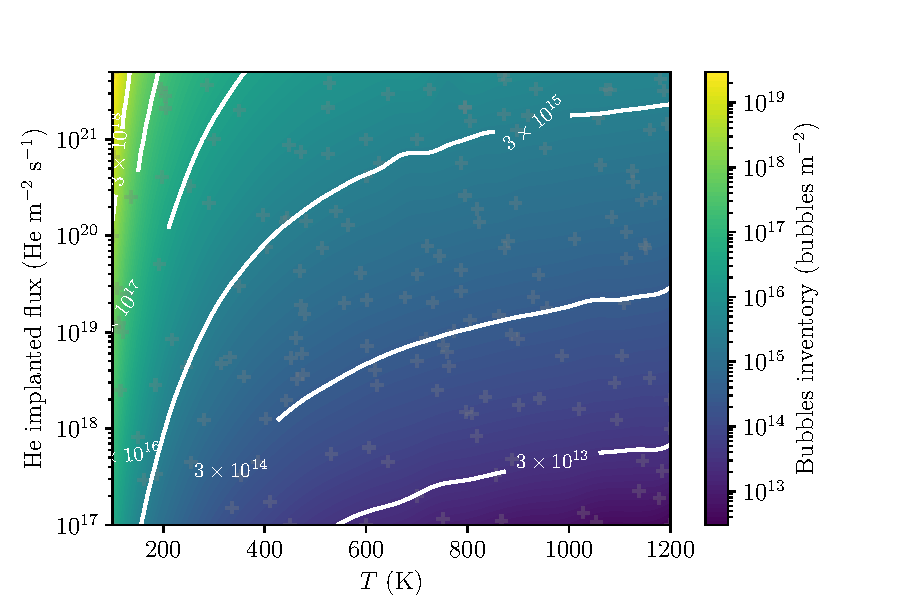
\includegraphics[width=\linewidth]{Figures/Chapter4/parametric study/bubbles_total_T_phi.pdf}
        \caption{Bubbles inventory $I_b = \int c_b \; dx$.}
        \labfig{inventory bubbles T phi}
    \end{subfigure}%
    \begin{subfigure}{0.5\linewidth}
        \centering
        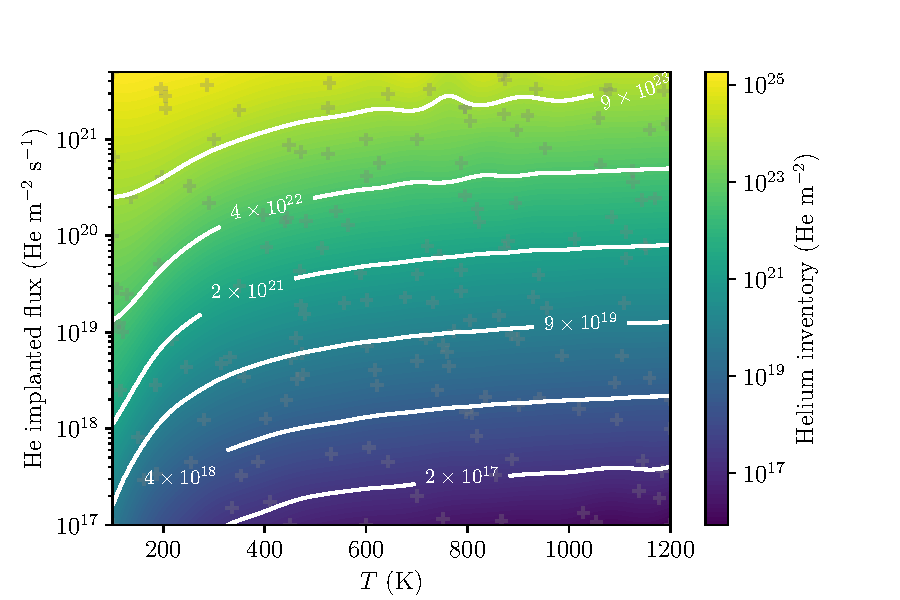
\includegraphics[width=\linewidth]{Figures/Chapter4/parametric study/inventory_T_phi.pdf}
        \caption{He inventory $I = \int \langle i_b \rangle c_b \; dx$.}
        \labfig{He inventory T phi}
    \end{subfigure}
    % \begin{subfigure}{0.5\linewidth}
    %     \centering
    %     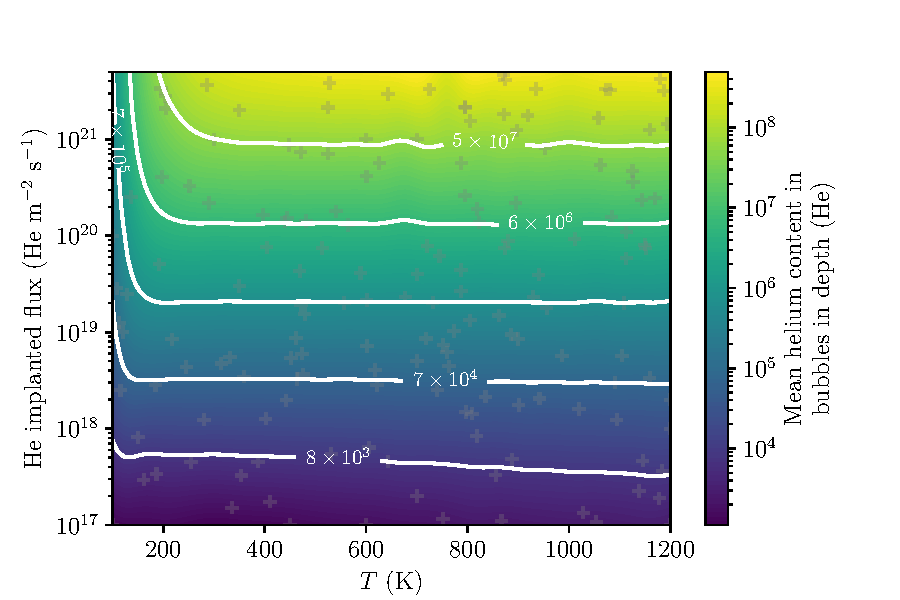
\includegraphics[width=\linewidth]{Figures/Chapter4/parametric study/mean_ib_T_phi.pdf}
    %     \caption{mean $\langle i_b \rangle$}
    % \end{subfigure}%
    % \begin{subfigure}{0.5\linewidth}
    %     \centering
    %     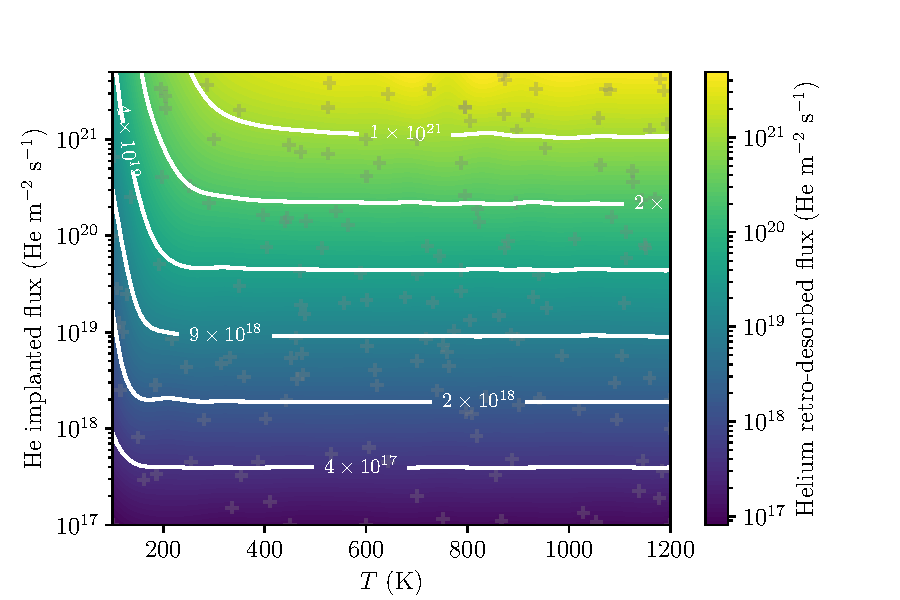
\includegraphics[width=\linewidth]{Figures/Chapter4/parametric study/surface_flux_T_phi.pdf}
    %     \caption{Retrodesorbed flux}
    % \end{subfigure}
    \begin{subfigure}{0.5\linewidth}
        \centering
        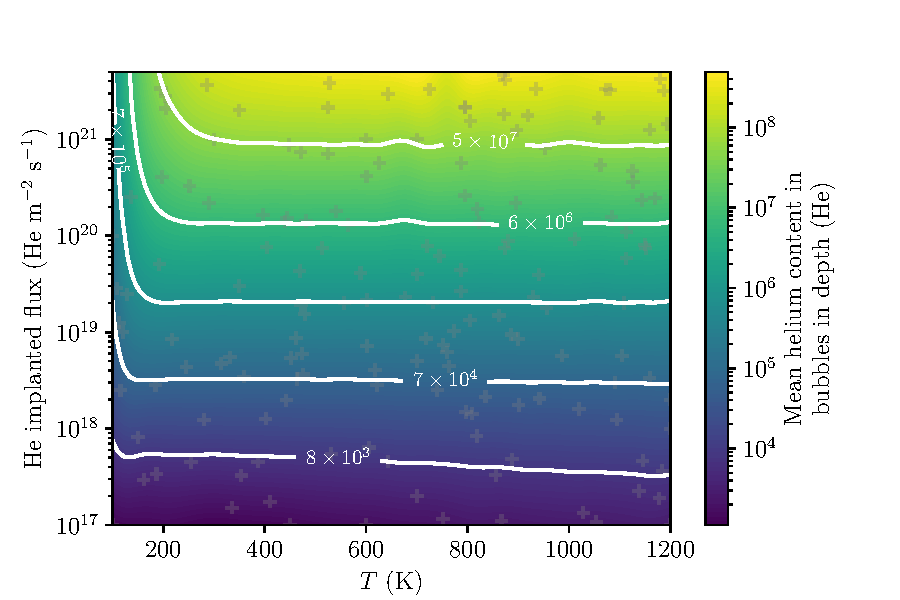
\includegraphics[width=\linewidth]{Figures/Chapter4/parametric study/mean_ib_T_phi.pdf}
        \caption{Average \gls{He} content in bubbles $\Bar{\langle i_b \rangle} = I / I_b$.}
        \labfig{mean ib T phi}
    \end{subfigure}%
    \begin{subfigure}{0.5\linewidth}
        \centering
        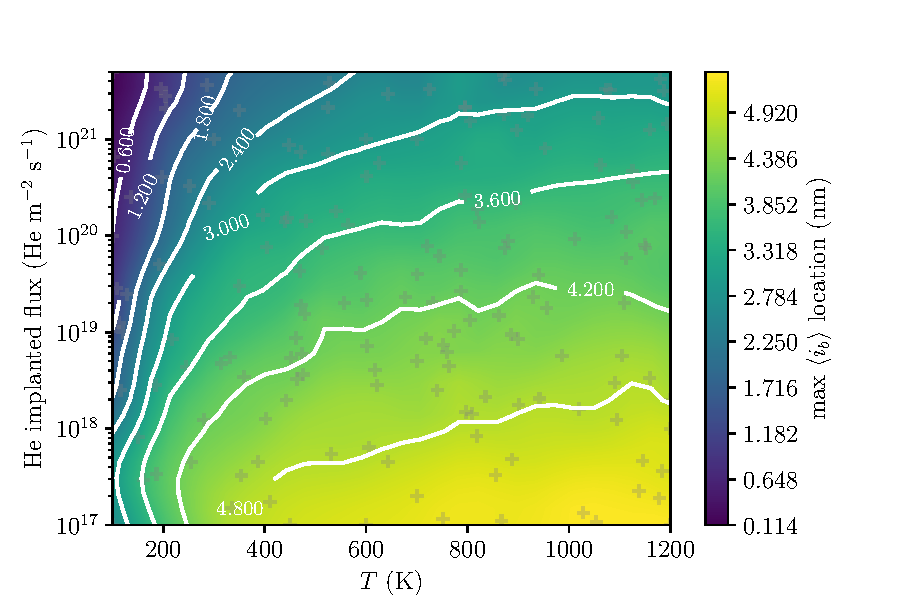
\includegraphics[width=\linewidth]{Figures/Chapter4/parametric study/x_max_ib_T_phi.pdf}
        \caption{Location of max $\langle i_b \rangle$.}
        \labfig{x max ib T phi}
    \end{subfigure}
    \caption{Evolution of quantities as a function of the implanted flux and temperature after \SI{1}{h} of \SI{100}{eV} \gls{He} exposure. Grey crosses correspond to simulations points.}
    \labfig{T phi quantities}
\end{figure*}

A parametric study was performed by varying the implanted flux $\varphi_\mathrm{imp}$ between \SI{1e17}{m^{-2} s^{-1}} and \SI{5e21}{m^{-2} s^{-1}} and the sample temperature $T$ between \SI{100}{K} and \SI{1200}{K}.

Several quantities were computed.
First the bubbles inventory is defined as:
\begin{equation}
    I_\mathrm{bubbles}= \displaystyle \int c_b \; dx
\end{equation}
The total helium inventory is calculated by:
\begin{equation}
        I = \displaystyle \int \sum\limits_{i=1}^N i c_i + \langle i_b \rangle c_b \; dx
        \approx \displaystyle \int \langle i_b \rangle c_b \; dx
    \labeq{I}
\end{equation}
The spatial mean helium content in bubbles can be computed as:
\begin{equation}
        \Bar{\langle i_b \rangle} = \frac{\displaystyle \int \langle i_b \rangle c_b \; dx}{\displaystyle \int c_b \; dx}
        \approx \frac{I}{I_\mathrm{bubbles}}
    \labeq{mean ib}
\end{equation}
The approximation made in \refeq{I} and \refeq{mean ib} is valid as long as $\int \langle i_b \rangle c_b dx \gg  \int \sum\limits_{i=1}^N i c_i dx$ (i.e.\ the He inventory is dominated by that of the bubbles).
This is the case in these simulations because $N=6$ (the influence of this parameter is discussed in \refsec{impact of N}).

More than 160 simulations were performed simulating \SI{1}{h} of exposure.
For each simulation, the quantities of interest described above were computed.
A Gaussian regression process \sidecite{chris_bowman_c-bowmaninference-tools_2020} was used to interpolate the data based on Bayesian inference as done in \sidecite{delaporte-mathurin_parametric_2020} (see \reffig{T phi quantities}).
The temporal evolution of these quantities was also assessed (see \reffig{quantities time}).

% bubbles inventory
After \SI{1}{h} of exposure, the bubbles inventory $I_\mathrm{bubbles}$ shows a weak dependence on temperature at high temperature and a weak dependence on the implanted flux at low temperature (see \reffig{inventory bubbles T phi}).
$I_\mathrm{bubbles}$ varies from \SI{4e12}{\text{bubbles } m^{-2}} at high temperature and low flux to \SI{2e19}{\text{bubbles } m^{-2}} at low temperature and high flux.

% He inventory
The \gls{He} inventory $I$ varies from \SI{8e16}{m^{-2}} at high temperature and low flux to \SI{e25}{m^{-2}} at low temperature and high flux (see \reffig{He inventory T phi}).
For temperatures above \SI{600}{K}, the temperature dependence is rather weak compared to the flux dependence.

% mean ib
For temperatures above \SI{300}{K}, and after \SI{1}{h} of exposure, the sample temperature does not impact the value of $\Bar{\langle i_b \rangle}$ (see \reffig{mean ib T phi}).
The mean He content increases with the implanted flux as expected and varies between \SI{e3}{He} at low flux and \SI{5e8}{He} at high flux.

% x max ib
The position of the maximum of $\langle i_b \rangle$ tended to increase with temperature and decrease with implanted flux (see \reffig{x max ib T phi}).
After \SI{1}{h} of exposure, it was found to be really close to the surface down to \SI{0.1}{nm} at low temperatures and high fluxes.
The validity of the model in this region of the parameter space is questionable considering that the bubble radius is greater that the thickness of the ligament between the edge of the bubble and the surface.
Such a bubble would therefore have burst before reaching this size. 

\begin{figure*} [ht!]
    \centering
    \begin{subfigure}{0.5\linewidth}
        \centering
        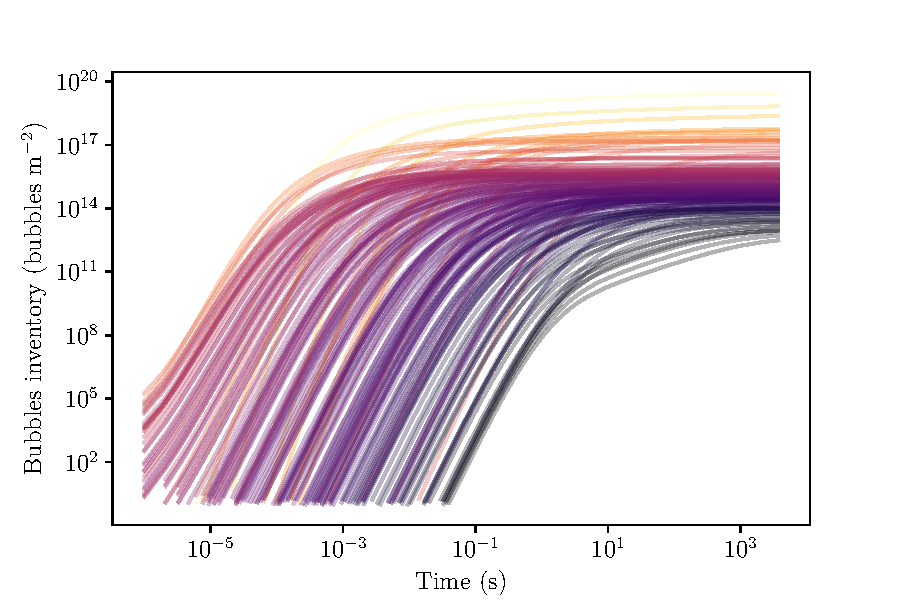
\includegraphics[width=\linewidth]{Figures/Chapter4/parametric study/total_bubbles_time.pdf}
        \caption{Bubbles inventory $I_b = \int c_b \; dx$.}
        \labfig{inventory bubbles time}
    \end{subfigure}%
    \begin{subfigure}{0.5\linewidth}
        \centering
        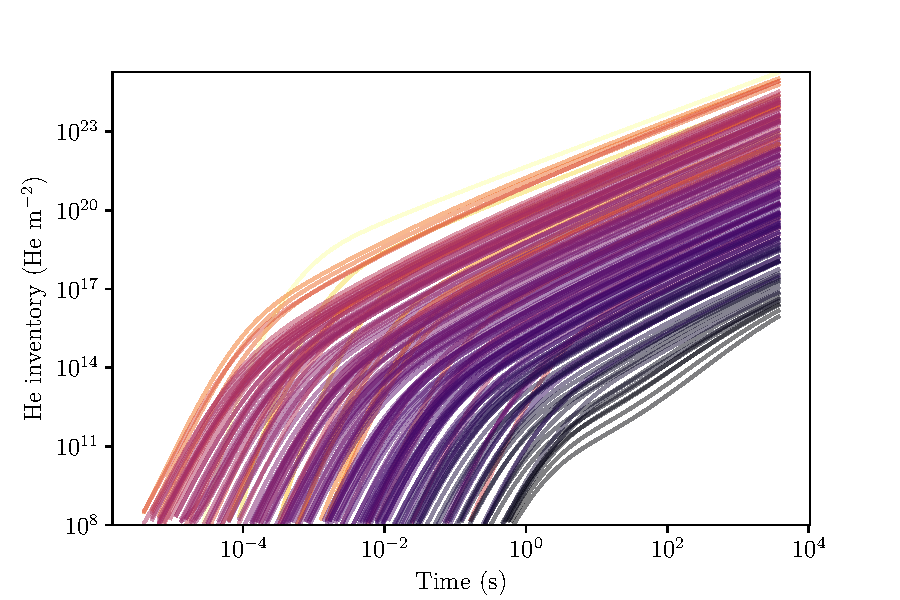
\includegraphics[width=\linewidth]{Figures/Chapter4/parametric study/inventory_time.pdf}
        \caption{He inventory $I = \int \langle i_b \rangle c_b \; dx$.}
        \labfig{He inventory time}
    \end{subfigure}
    % \begin{subfigure}{0.5\linewidth}
    %     \centering
    %     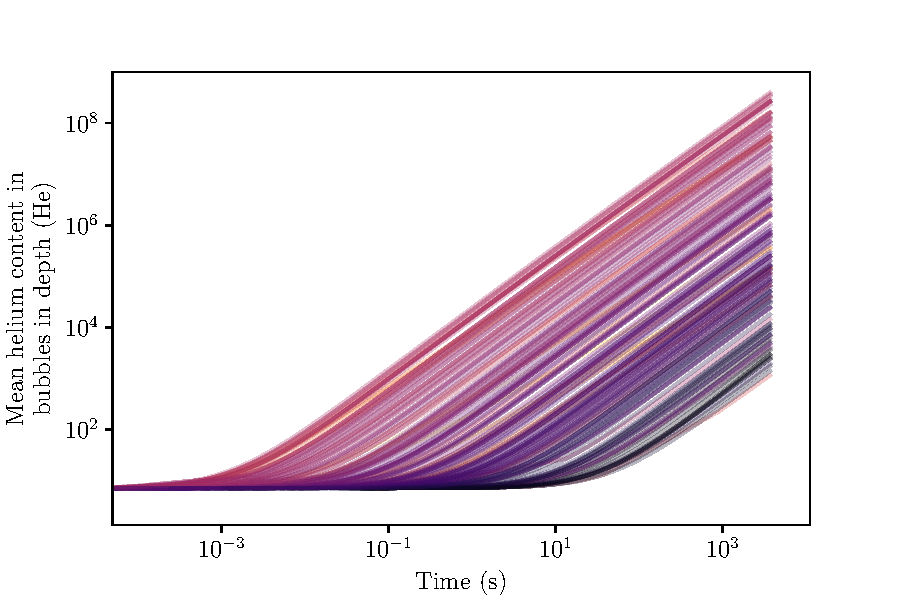
\includegraphics[width=\linewidth]{Figures/Chapter4/parametric study/mean_ib_time.pdf}
    %     \caption{mean $\langle i_b \rangle$}
    % \end{subfigure}%
    % \begin{subfigure}{0.5\linewidth}
    %     \centering
    %     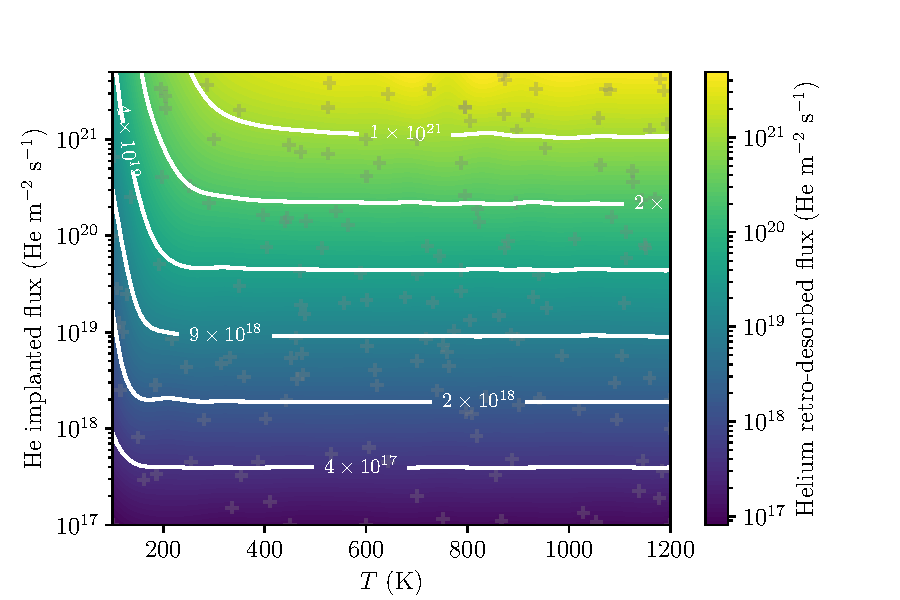
\includegraphics[width=\linewidth]{Figures/Chapter4/parametric study/surface_flux_T_phi.pdf}
    %     \caption{Retrodesorbed flux}
    % \end{subfigure}
    \begin{subfigure}{0.5\linewidth}
        \centering
        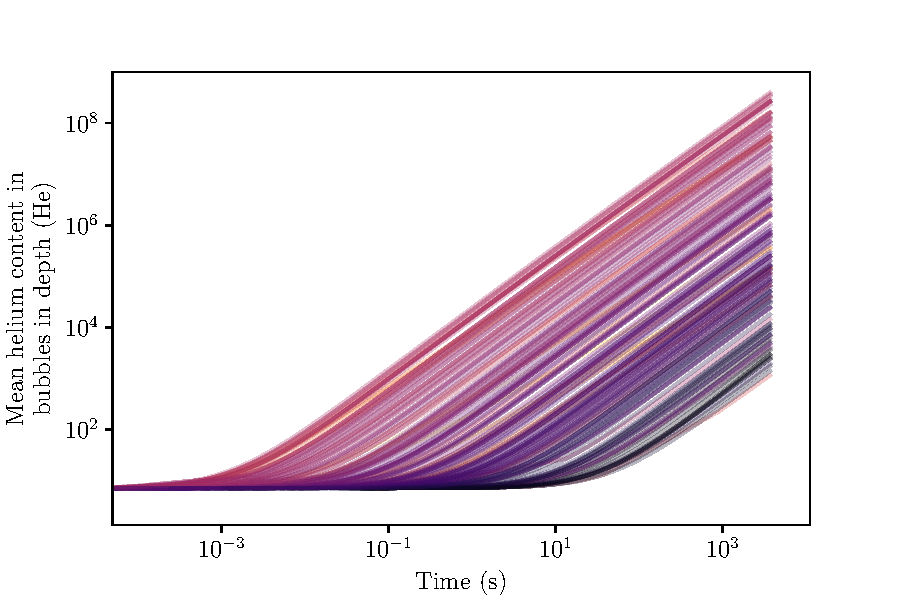
\includegraphics[width=\linewidth]{Figures/Chapter4/parametric study/mean_ib_time.pdf}
        \caption{Average He content in bubbles $\Bar{\langle i_b \rangle} = I / I_b$.}
        \labfig{mean ib time}
    \end{subfigure}%
    % \begin{subfigure}{0.5\linewidth}
    %     \centering
    %     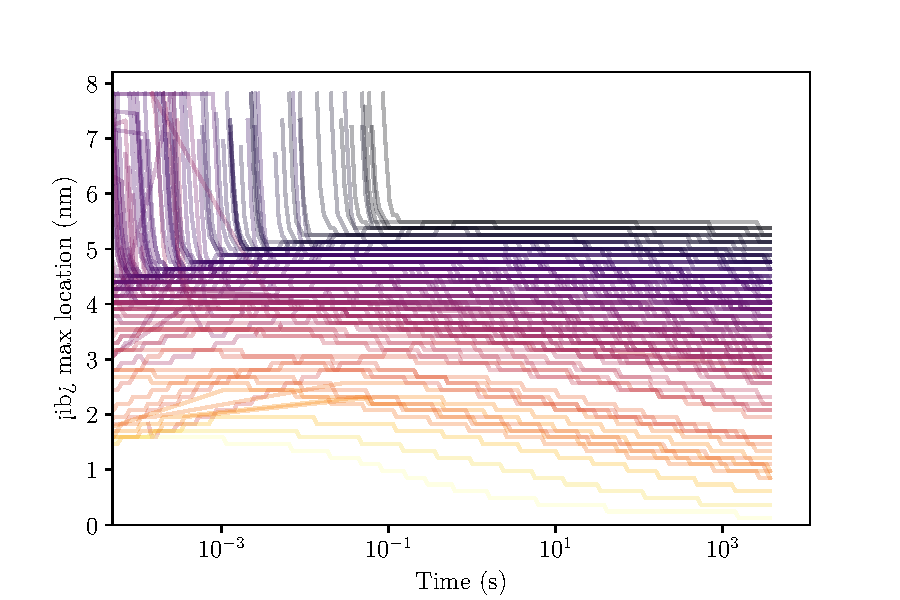
\includegraphics[width=\linewidth]{Figures/Chapter4/parametric study/x_max_ib_time.pdf}
    %     \caption{x max $\langle i_b \rangle$}
    %     \labfig{x max ib time}
    % \end{subfigure}
    \begin{subfigure}{0.5\linewidth}
        \centering
        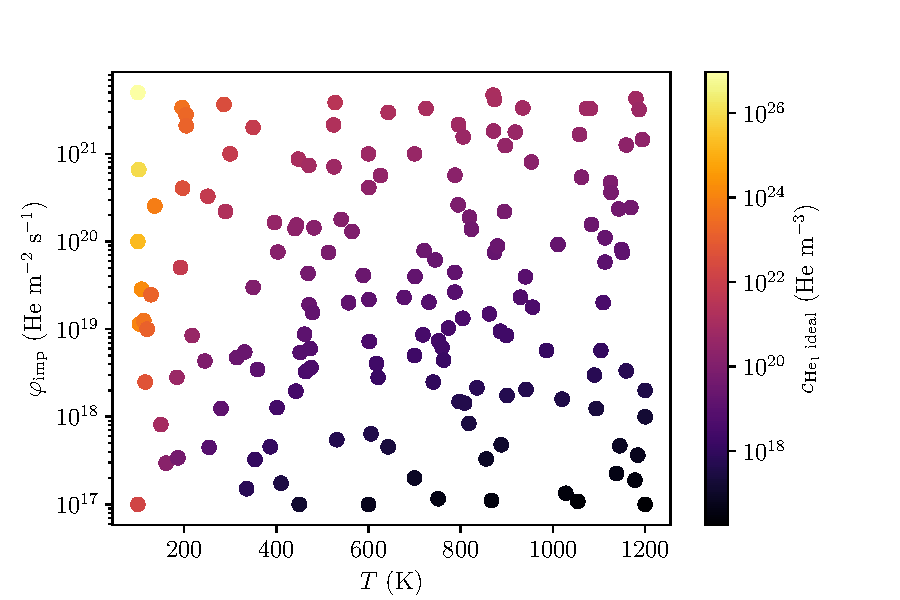
\includegraphics[width=\linewidth]{Figures/Chapter4/parametric study/points_with_parameter.pdf}
        \caption{Simulation points coloured according to $c_{\mathrm{He}_1, \mathrm{ideal}}$.}
        \labfig{simulations points with parameter}
    \end{subfigure}
    \caption{Temporal evolution of quantities in W exposed to \SI{100}{eV} He at \SI{e22}{m^{-2}.s^{-1}} and \SI{1000}{K} for temperatures varying from \SI{120}{K} to \SI{1200}{K} and implanted fluxes varying from \SI{e17}{m^{-2}s^{-1}} to \SI{e21}{m^{-2}s^{-1}}. Each line corresponds to a simulation point (grey crosses on \reffig{inventory bubbles T phi} and points on \reffig{simulations points with parameter}). The lines are coloured according to the parameter $c_{\mathrm{He}_1, \mathrm{ideal}} = \varphi_\mathrm{imp} \; R_p/D(T)$ with $R_p = \SI{1.5}{nm}$ and $D$ the diffusion coefficient of $\mathrm{He}_1$ in W.}
    \labfig{quantities time}
\end{figure*}

% time series
For each simulation point, the temporal evolution of the quantities described above has been computed.
To better identify the time series on the $\varphi_\mathrm{imp}, T$ plane, lines have been coloured according to the parameter $c_{\mathrm{He}_1, \mathrm{ideal}}$ which is a function of both the implanted flux and the temperature (see \refeq{c he1 ideal}) expressed in \si{m ^{-3}}.

\begin{equation}
    c_{\mathrm{He}_1, \mathrm{ideal}} = \frac{\varphi_\mathrm{imp} \; R_p}{D(T)}
    \labeq{c he1 ideal}
\end{equation}
where $\varphi_\mathrm{imp}$ is the implanted flux, $D$ is the diffusion coefficient of mobile $\mathrm{He}_1$ in W (see \reftab{clusters properties}), $R_p = \SI{1.5}{nm}$ is the implantation depth and $T$ is the temperature in \si{K}.

All these quantities showed a similar behaviour in time even though the kinetics were found to be different (see \reffig{quantities time}).
For instance, for each $(T, \varphi_\mathrm{imp})$ couple, $I_\mathrm{bubbles}$ first increased as a power law of time before reaching a maximum (see \reffig{inventory bubbles time}).
The total He inventory $I$ increased with time and for each simulation point, but the growth rate decreased at long exposure times (see \reffig{He inventory time}).
This phenomenon is explained in details in \refsec{nucleation growth phases}.
Similarly, $\Bar{\langle i_b \rangle}$ could be written as a power law of time described in Eq \refeq{ib evolution} (see \reffig{mean ib time}).
The depth of the maximum of $\langle i_b \rangle$ tended to decrease with time as it was observed in \refsec{half slab} (see \reffig{inventory bubbles time}).

\subsubsection{Inventory evolution regimes} \labsec{nucleation growth phases}

\begin{figure} [h]
    \centering
    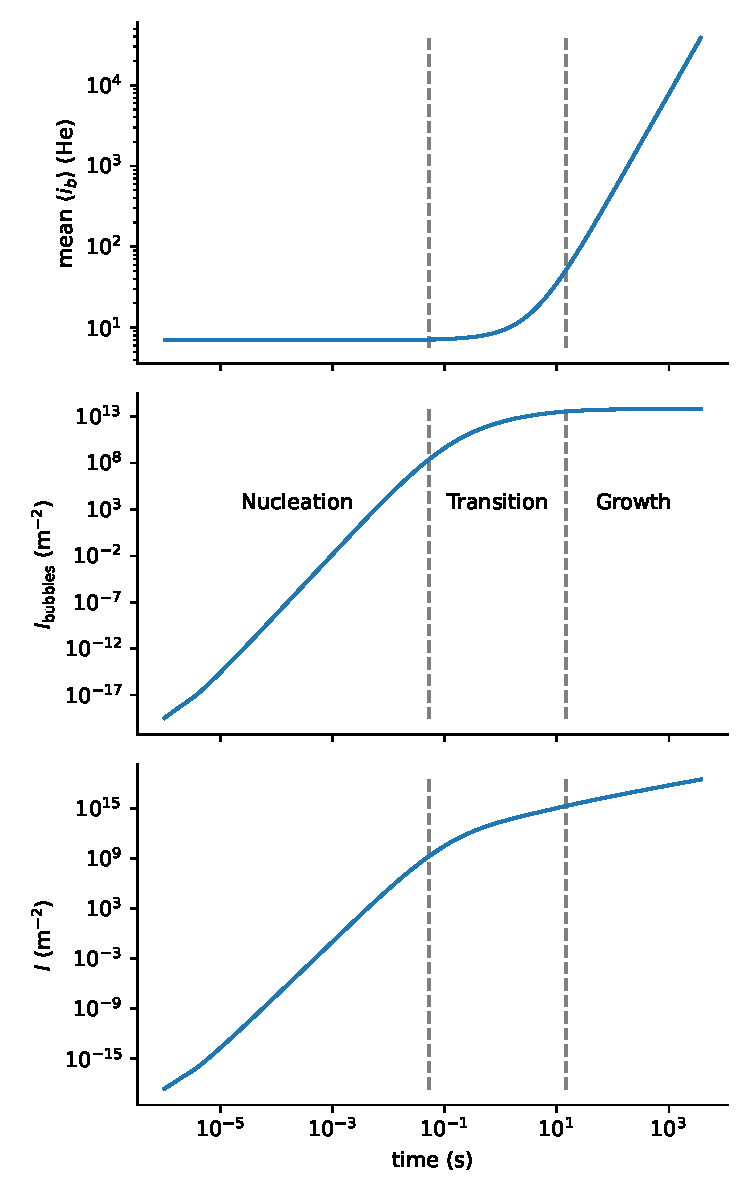
\includegraphics[width=0.75\linewidth]{Figures/Chapter4/parametric study/inventory_bubbles_ib.pdf}
    \caption{Temporal evolution of $\Bar{\langle i_b \rangle}$, $I_\mathrm{bubbles}$ and $I$ in W exposed to \SI{100}{eV} He at \SI{1.59e18}{m^{-2}.s^{-1}} and \SI{1020}{K}. The dashed grey vertical line represents the transition from nucleation regime to bubble growth regime.}
    \labfig{two regimes}
\end{figure}

For every $(T, \varphi_\mathrm{imp})$ couple, $I_\mathrm{bubbles}$ increased rapidly at low \glspl{fluence} until reaching a maximum at high \glspl{fluence} (see \reffig{inventory bubbles time}).
On the other hand, the mean \gls{He} content $\Bar{\langle i_b \rangle}$ was constant at low \glspl{fluence} and increased as a power law of time at high \glspl{fluence} (see \reffig{mean ib time}).
The evolution of $\Bar{\langle i_b \rangle}$ can be described as:
\begin{equation}
    \Bar{\langle i_b \rangle} = N + 1 + a \; t^b
    \labeq{ib evolution}
\end{equation}
where $N=6$ in this model, $a$ and $b$ depend on $(T, \varphi_\mathrm{imp})$.
The choice of $N=6$ in this model is detailed in \refsec{impact of N}.
The total \gls{He} \gls{inventory} $I$ being the product of these two quantities, two different growth rates were observed (see \reffig{He inventory time} and \reffig{two regimes}).

This phenomenon can be attributed to two different regimes.
The first regime is the nucleation regime where new bubbles nucleons are created (i.e.\ $c_b$ and $I_\mathrm{bubbles}$ increase).
In the nucleation regime, the bubble concentration $c_b$ and the capture radius $\langle r_b \rangle$ are too low for the He content in bubbles $\langle i_b \rangle$ to increase significantly (i.e.\ $\Bar{\langle i_b \rangle}$ is constant).
The second regime is the bubble growth regime.
In this regime, $c_b$ is high enough for interactions between bubbles and mobile He to occur.
Implanted interstitial He atoms ($c_{\mathrm{He}_1}$) therefore interact preferably with bubbles rather than clustering with other interstitial He atoms.
This means that no additional bubbles nucleons are created (i.e.\ $c_b$ reaches a maximum).
Because interactions between bubbles and mobile He are strong, the term $\langle k_b^+ \rangle c_1 c_b$ in \refeq{temporal evolution grouping} becomes significant and the He content increases (i.e.\ $\Bar{\langle i_b \rangle}$ increases).
This is illustrated by the thickness of the arrows in \reffig{clustering sketch}.


\subsubsection{Influence of $N$} \labsec{impact of N}
In order to assess the impact of the parameter $N$ in \refeq{temporal evolution grouping}, the evolution of the He inventory $I$, the mean He content in immobile clusters (different from $\Bar{\langle i_b \rangle}$) and the bubbles inventory $I_\mathrm{bubbles}$ was computed with several values of $N$.

The flux of \SI{100}{eV} He in this test case was \SI{e20}{m^{-2} s^{-1}} and the temperature was \SI{1000}{K}. 

It was shown that varying $N$ had no impact on these quantities whatsoever (see \reffig{N variation}).
This highlights the very quick transition from nucleation regime to growth regime in this model.

The number of equations that need to be solved can therefore be minimised by setting the parameter $N$ to its minimum ($N=6$) without losing accuracy in the results.
This minimum value corresponds to the number of mobile clusters which have to be explicitly simulated in order to account for all the diffusion mechanisms.

\begin{figure} [h]
    \centering
    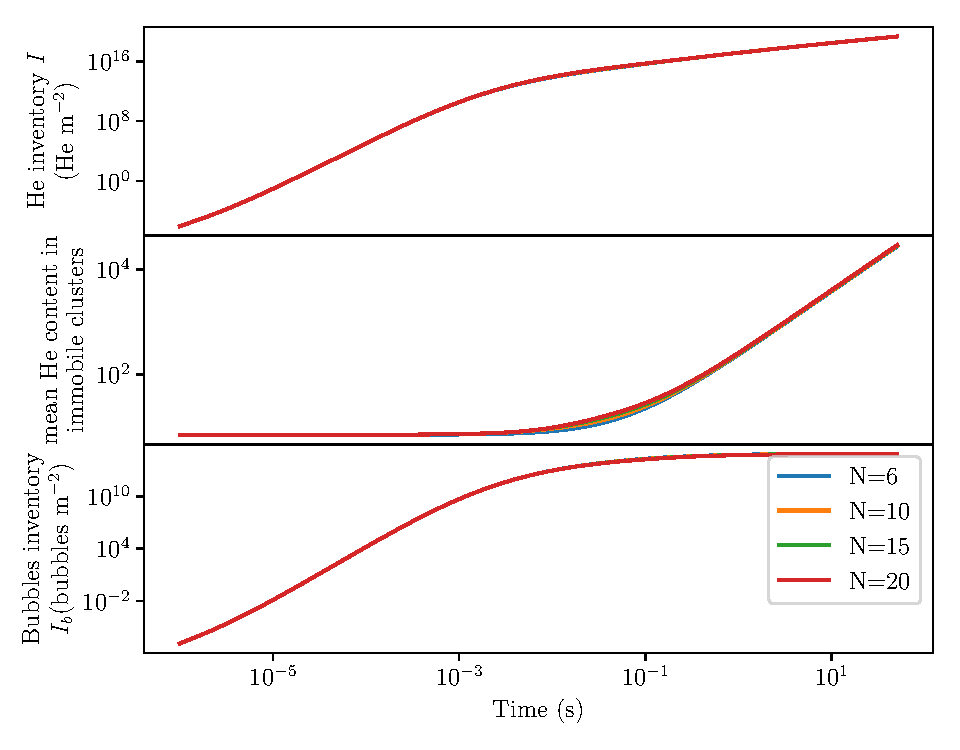
\includegraphics[width=\linewidth]{Figures/Chapter4/varying_N.pdf}
    \caption{Comparison of several quantities of interest for several values of $N$ in W exposed to \SI{100}{eV} He at \SI{e20}{m^{-2}.s^{-1}} and \SI{1000}{K}.}
    \labfig{N variation}
\end{figure}


\section{Influence on hydrogen transport}
The focus of this Section is the coupled effects of \gls{He} implantation and hydrogen transport.
To this end, the experiment of Ialovega and co-workers \sidecite{ialovega_hydrogen_2020} is reproduced with the \gls{He} bubble model described in this Chapter coupled to FESTIM.

\subsection{Experiment and FESTIM simulation description}

A \SI{100}{\micro\metre} thick tungsten sample was pre-damaged with \SI{75}{eV} He at \SI{1073}{K}.
The \gls{He} flux was \SI{2.3e22}{m^{-2}.s^{-1}} and the exposure time was \SI{13}{s}.
An initial cleaning \gls{tds} was performed up to \SI{870}{K}.

Sequential deuterium loading and \gls{tds} were then repeated five times.
\SI{250}{eV} deuterium were implanted at room temperature with a flux of \SI{1.7e16}{m^{-2}.s^{-1}} and a \gls{fluence} of \SI{4.5e19}{m^{-2}}.
The \gls{tds} phase ramps up to \SI{1350}{K} (\SI{1250}{K} for the first \gls{tds}) at a rate of \SI{1}{K.s^{-1}}.

Four traps are simulated: traps 1-3 are pre-existing defects and trap 4 represents the traps induced by \gls{He} bubbles.
The detrapping energies and trap densities are set as free parameters, including the trap density $n_b$ (see \reftab{trap properties}).

Considering deuterium is trapped on the surface of \gls{He} bubbles, the bubble trap density $n_b$ is given by:

\begin{equation}
    n_b = f \cdot c_b \cdot \Ab(\langle r_b \rangle)
\end{equation}
where $f$ is a free parameter representing the number of trapping site per unit surface, $\Ab = 4\pi \langle r_b \rangle^2$ is the area in \si{m^2} of a spherical bubble of radius $\langle r_b \rangle$, and $c_b$ is the concentration of bubbles in $\si{m^{-3}}$.

The quantities $c_b$ and $\langle r_b \rangle$ have been computed from the model described in \refsec{helium model description} (see \reffig{trap bubbles distribution}).

\begin{figure}[h!]
    \centering
    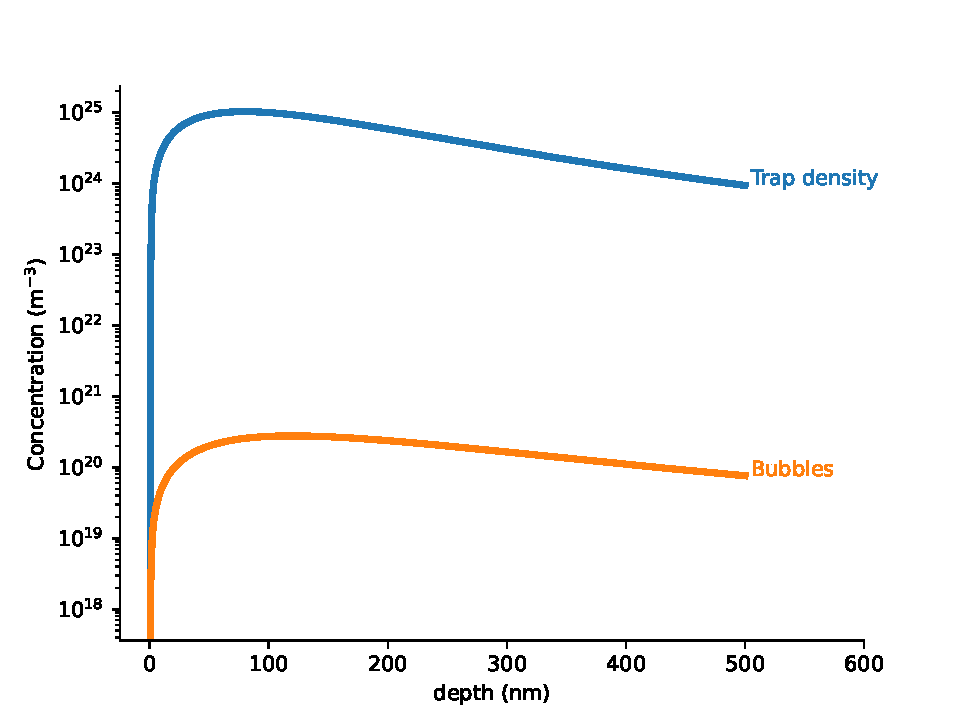
\includegraphics[width=\linewidth]{Figures/Chapter5/trap_bubble_distribution.pdf}
    \caption{Spatial distribution of the bubbles density and the equivalent trap density (assuming $f=\SI{3e18}{m^{-2}}$).}
    \labfig{trap bubbles distribution}
\end{figure}


\begin{table}[!h]
    \caption{Trap properties used to fit the TDS spectra. The density distribution $n_b$ as well as detrapping energies $E_p$ are assumed constant across TDS experiments.}
    \begin{tabular}{r l l l l l}
    \\
     & $k_0$ & $E_k$ & $p_0$ & $E_p$ & $n$ \\
     \ & [\si{m^{3}.s{-1}}] & [\si{eV}] & [\si{s^{-1}}] & [\si{eV}] & [\si{m^{-3}}] \\
    \\
    Trap 1 & \multirow{7}{*} { $9 \times 10 ^{-17}$ } & \multirow{7}{*} { 0.39 } & \multirow{7}{*} { $10^{13}$ } & free & free \\
    \\
    Trap 2 & & & & free & free \\
    \\
    Trap 3 & & & & free & free \\
    \\
    Trap bubbles & & & & free & $n_b$ \\
    \end{tabular}
    \labtab{trap properties}
\end{table}

The diffusion coefficient of deuterium (\si{m^2.s^{-1}}) was set to $4.1\times 10 ^{-7} \exp{-0.39/k_B T}$ \sidecite{frauenfelder_solution_1969}.
The \SI{250}{eV} deuterium implantation was represented by a Gaussian distrubiton with a mean implantation depth \SI{10}{nm} and a standard deviation of \SI{4.5}{nm} (calculated from SRIM \sidecite{ziegler_srim_2010}).
Finally, an instantaneous recombination was assumed on the surfaces.

Using the parametric optimisation method developed in \sidecite{delaporte-mathurin_parametric_2021}, the free parameters are identified.

\subsection{Results}

The properties obtained by the fitting procedure (see \reftab{trap properties results}) fitted well the three \gls{tds} spectra (see \reffig{fitted TDS}).
As explained in \cite{ialovega_hydrogen_2020}, the last bump of desorption (around \SI{600}{K}) is due to a temperature control issue and was therefore ignored in the fitting procedure.
The detrapping energies of traps 1, 2 and 3 were found to be \SI{1.08}{eV}, \SI{1.20}{eV} and \SI{1.38}{eV} respectively, whereas the trap attributed to \gls{He} bubbles has a detrapping energy of \SI{1.45}{eV}.


\begin{table}[!h]
    \caption{Results of the fitting procedure. Detrapping energies $E_p$ are given in \si{eV}, trap densities in \si{at.fr.} and $f$ in \si{m^{-2}}.}
    \begin{tabular}{r l l l l l l l l}
    \\
    &\multicolumn{2}{l}{Trap 1}  & \multicolumn{2}{l}{Trap 2} & \multicolumn{2}{l}{Trap 3} &\multicolumn{2}{l}{Trap bubbles} \\
     & $E_p$ & $n$ ($\times 10 ^{-3}$) & $E_p$ & $n$ ($\times 10 ^{-3}$) & $E_p$ & $n$ ($\times 10 ^{-3}$) & $E_p$ & $f$ ($\times 10 ^{18}$) \\
    \\
    1st \gls{tds} & - & 0.00 & - & 0.00 & - & 0.00 & 1.42 & $3.00$ \\
    \\
    2nd \gls{tds} & 1.08 & $2.20$ & 1.20 & $1.80$ & 1.37 & $2.00$ & 1.42 & $3.00$ \\
    \\
    5th \gls{tds} & 1.08 & $3.38$ & 1.20 & $3.10$ & 1.37 & $1.50$ & 1.42 & $3.00$ \\
    \end{tabular}
    \labtab{trap properties results}
\end{table}

This would mean that if the \gls{tds} were run up to temperature around \SI{1600}{K}, $\mathrm{He}_1\mathrm{V}_1$ clusters could dissociate resulting in additional free trapping sites for \gls{H} and therefore different \gls{tds} spectra.

The \gls{H} retention is not dominated by \gls{He}-bubbles trapping but rather by pre-existing defects.

\begin{figure}[h!]
    \centering
    \begin{subfigure}{\linewidth}
        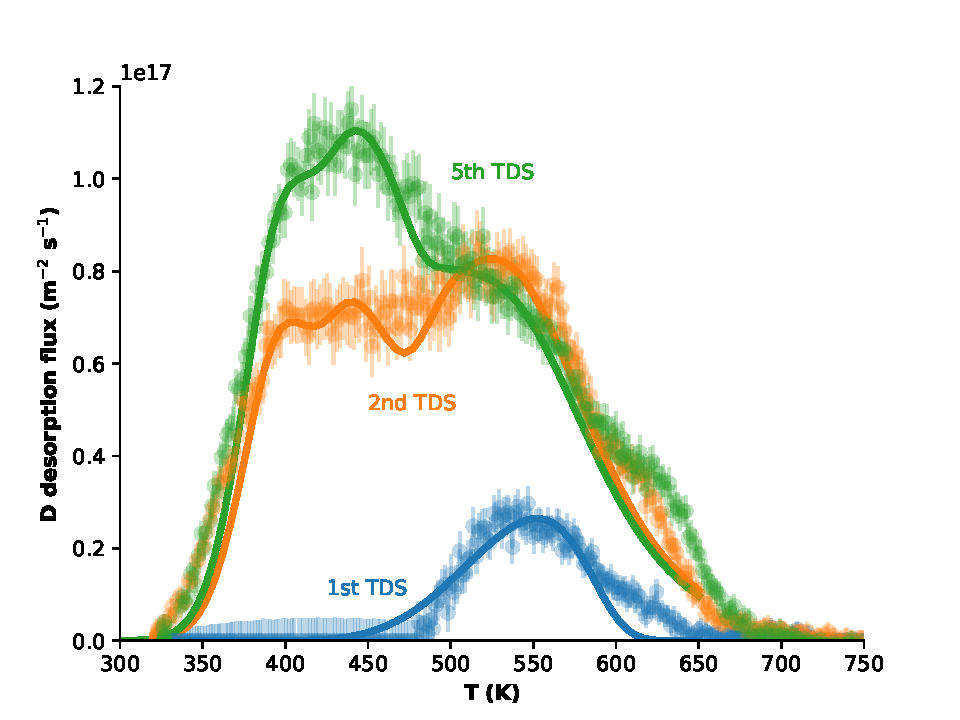
\includegraphics[width=\linewidth]{Figures/Chapter5/ialovega_tds.pdf}
        \caption{Experimental TDS spectra fitted with FESTIM. Experimental points are taken from \cite{ialovega_hydrogen_2020}.}
        \labfig{3 TDS}
    \end{subfigure}
    \begin{subfigure}{\linewidth}
        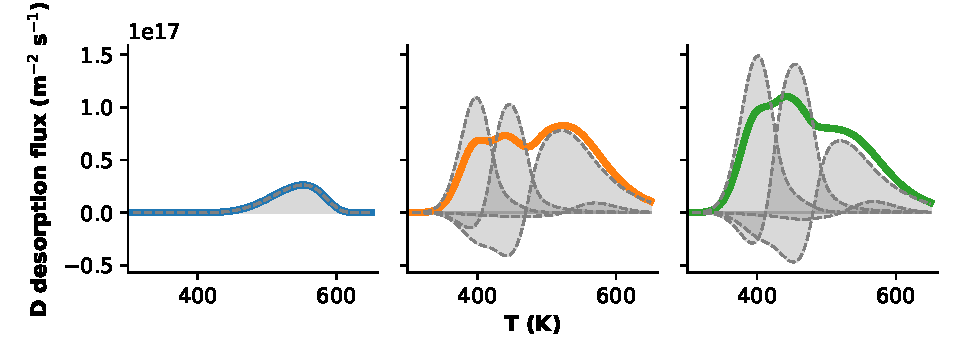
\includegraphics[width=\linewidth]{Figures/Chapter5/tds_trap_distribution.pdf}
        \caption{Traps contribution to the TDS spectra.}
        \labfig{trap contributions}
    \end{subfigure}
    \caption{Results of the TDS fitting procedure.}
    \labfig{fitted TDS}
\end{figure}

\begin{figure}
    \centering
    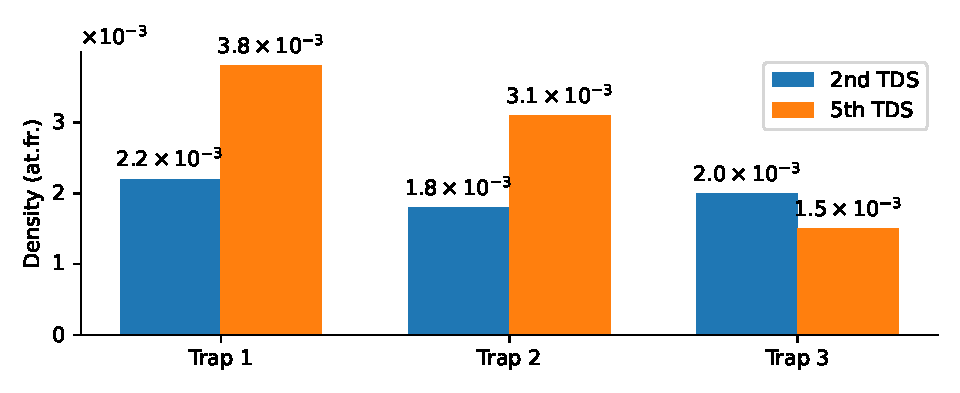
\includegraphics[width=\linewidth]{Figures/Chapter5/trap_densities.pdf}
    \caption{Evolution of the trap densities between the second and fifth TDS.}
    \labfig{density evolution}
\end{figure}

The densities of traps 1 and 2 increased from the 2nd to the 5th \gls{tds} (see \reffig{density evolution}).
However, the density of trap 3 decreased slightly (which is also visible on the \gls{tds} spectra shown in \reffig{fitted TDS}).
The processes at stake cannot yet be precisely described. 

One possible interpretation of the results is:
\begin{itemize}
    \item Initial state: the sample has some pre-existing defects %(proof from PAS that there are pre-existing defects before He implantation)
    \item \gls{He} implantation: all pre-existing defects are saturated with \gls{He} and bubbles are formed
    \item 1st D implantation: D can only be trapped around bubbles since defects are saturated with \gls{He}
    \item 1st \gls{tds} (up to \SI{1250}{K}): D is detrapped from bubbles is desorbed (\SI{550}{K} peak), \gls{He} dissociates from pre-existing defects 
    \item 2nd D implantation: D is trapped around bubbles and in the non-saturated defects
    \item 2nd \gls{tds} (up to \SI{1350}{K}): D is detrapped from bubbles is desorbed (\SI{550}{K} peak) and from non-saturated defects (peaks 400K, 450K and 500K) + \gls{He} trapped in deeper traps dissociate (because the \gls{tds} goes to higher temperatures)
    \item 3rd to 5th D implantations: D is trapped around bubbles and in pre-existing defects
    \item 3rd to 5th \gls{tds}: D is detrapped from bubbles and pre-existing defects (now more available than at the 2nd \gls{tds})
\end{itemize}
This interpretation is represented (in a simplified way) on \reffig{ialovega experiment interpretation}.


\begin{figure*}
    \centering
    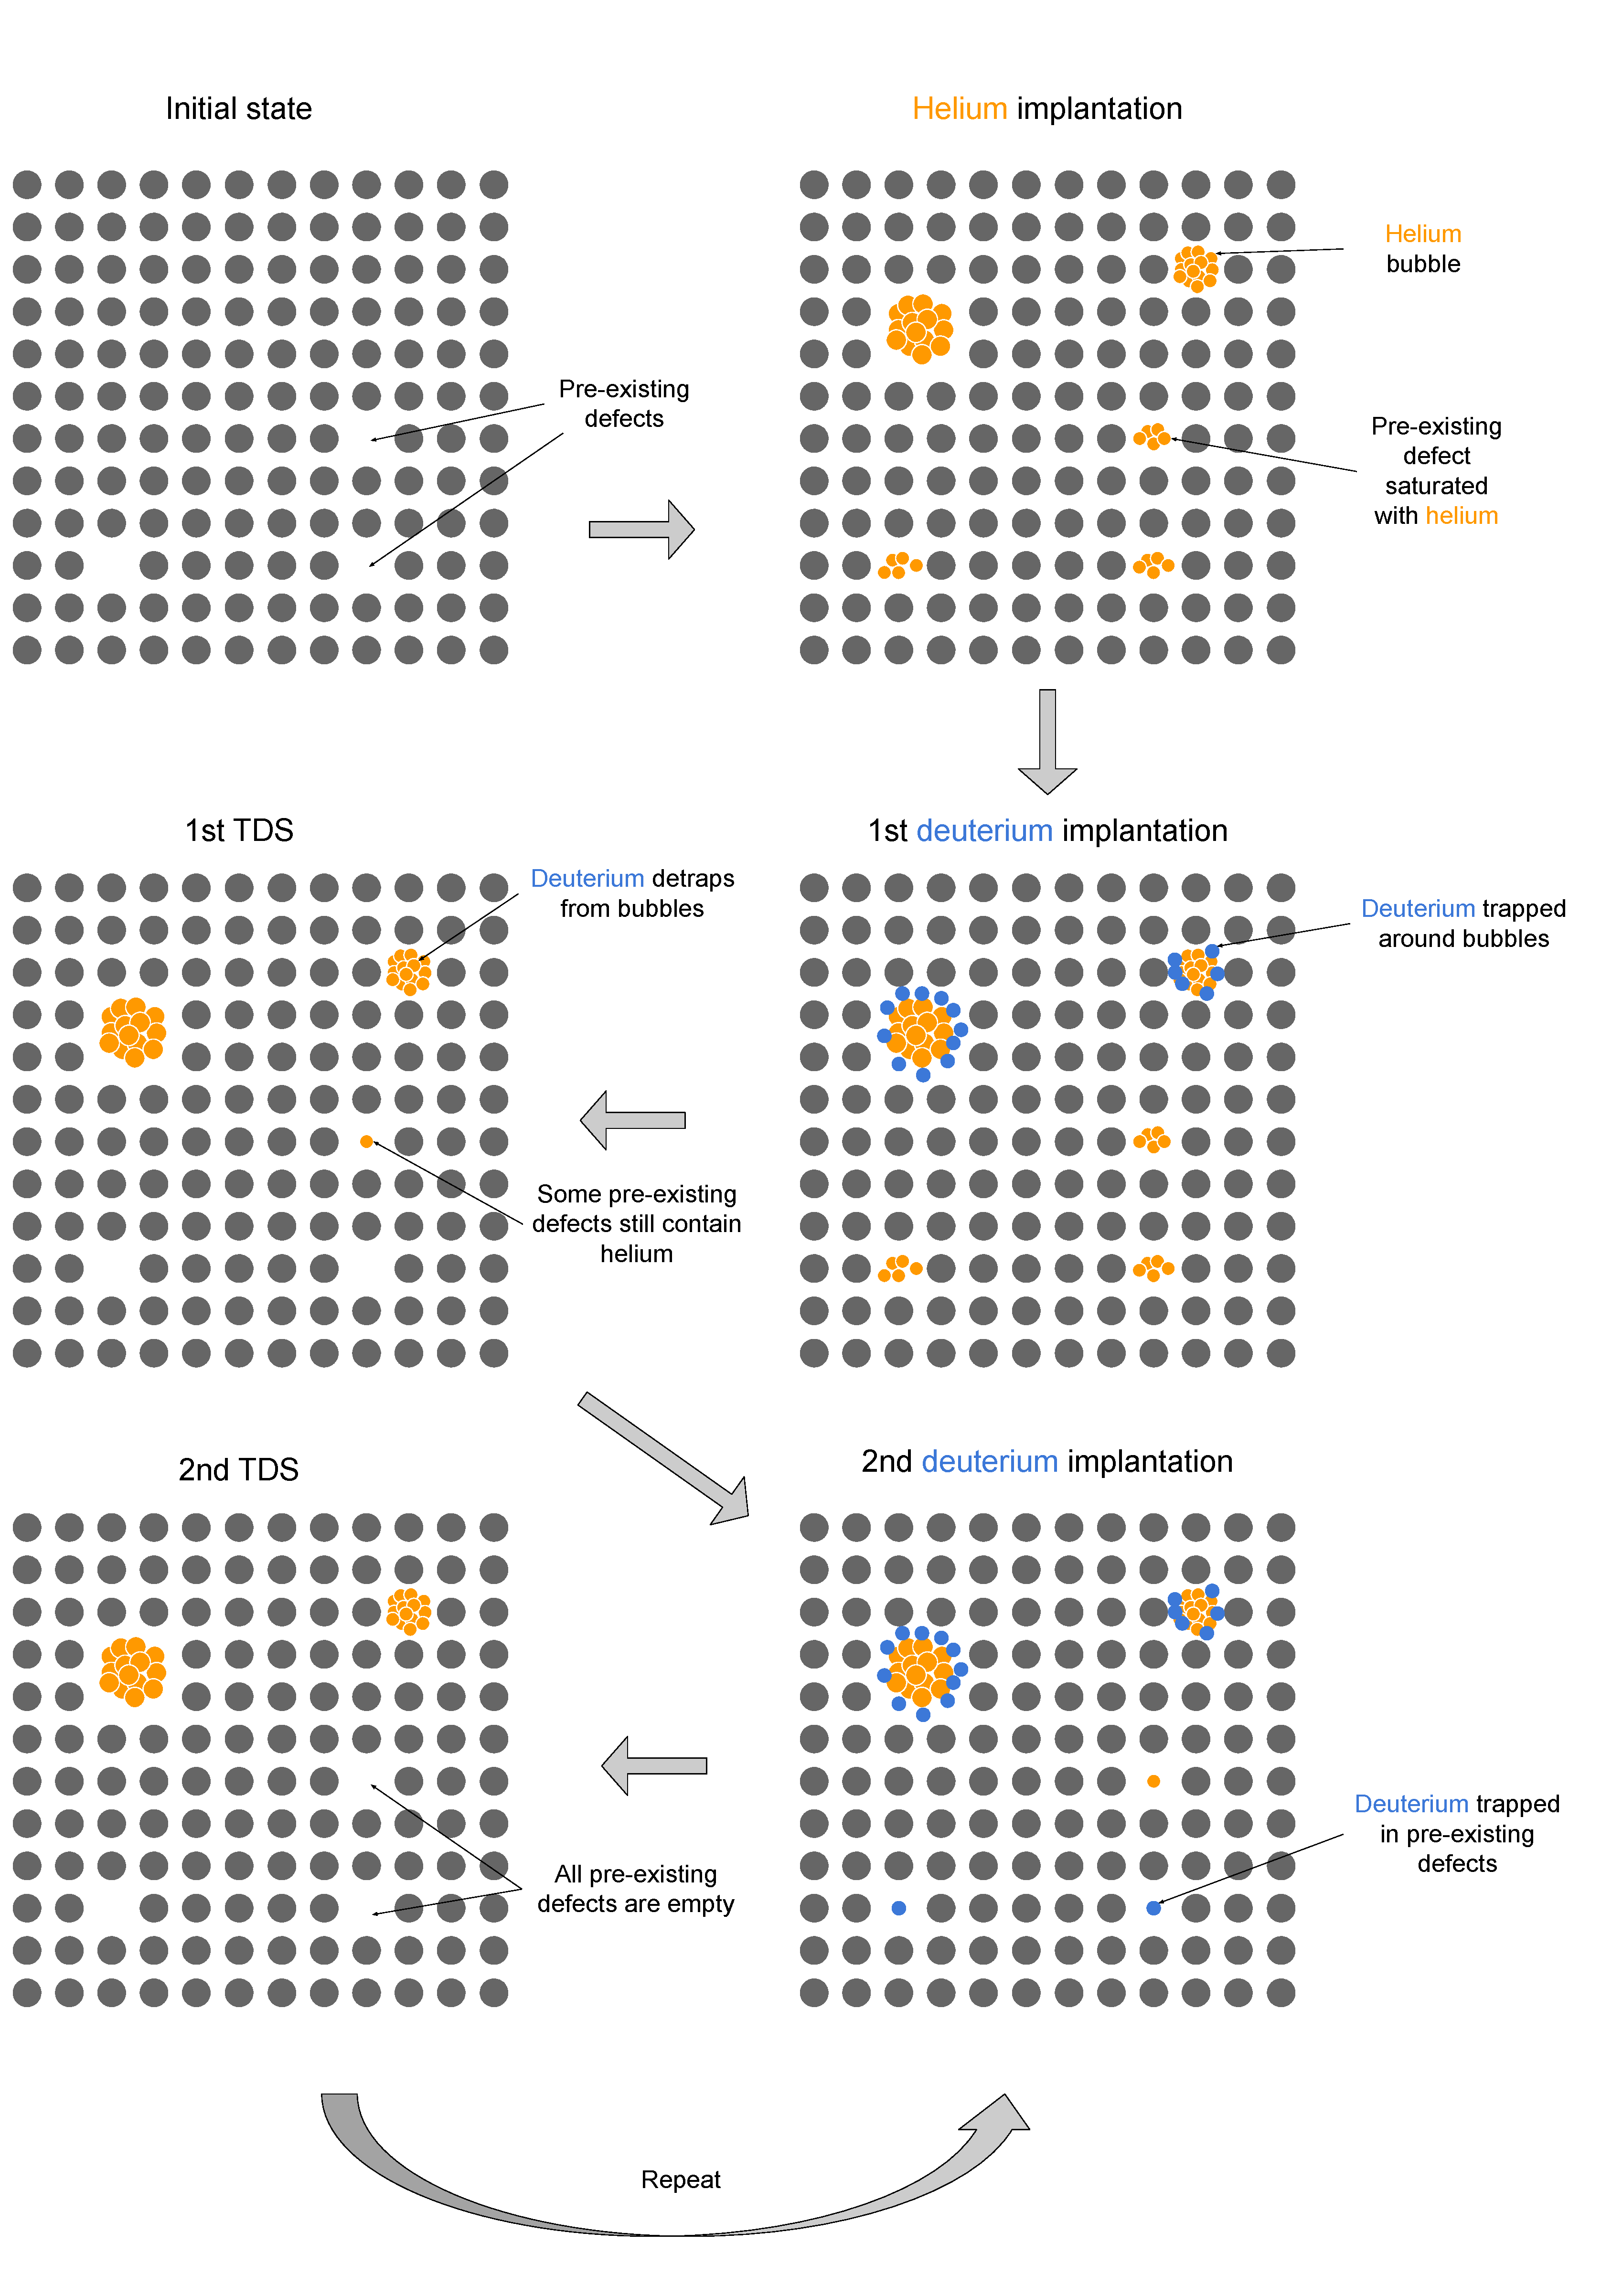
\includegraphics[width=\linewidth]{Figures/Chapter5/sketch ialovega experiment.pdf}
    \caption{Schematic interpretation of the simulation results showing the several stages of the experiment (from \gls{He} implantation to TDS cycles).}
    \labfig{ialovega experiment interpretation}
\end{figure*}


\section{Summary}

\gls{festim} was used to simulate the influence of helium implantation on hydrogen transport.
The formation of helium bubble in tungsten was first studied.
It was shown that this phenomenon was limited to a small region near the exposed surface.

The experiment of Ialovega and co-workers described in \sidecite{ialovega_hydrogen_2020} was then reproduced and one possible explanation was given.
Although fitting a \gls{tds} spectrum is not sufficient to draw strong conclusions, this work suggests that:
\begin{itemize}
    \item helium does not leave bubbles in significant quantities at these temperatures
    \item helium occupies pre-existing defects avoiding hydrogen to get trapped
    \item Hydrogen retention is not dominated by helium-induced bubbles but rather by the saturation of pre-existing defects by helium
\end{itemize}

From these results, several experimental suggestions can be made.
Running the \gls{tds} up to \SI{750}{K} only would limit helium desorption.
Indeed, it was shown in \cite{ialovega_hydrogen_2020} that there was no helium desorption below this temperature after the initial cleaning \gls{tds}.
If helium does not desorb and remains in the pre-existing defects, the deuterium \gls{tds} spectra should not be affected and only the desorption from bubbles should be observed.
This would confirm or infirm the interpretation of the results presented herein.

Moreover, if this interpretation was confirmed, it could have implications for hydrogen retention.
Indeed, one could imagine reducing the tritium inventory of components by first exposing them to helium.
Helium would fill the existing defects, making it impossible for tritium to be trapped.
However, having a helium inventory in components can also have negative consequences.
